\thispagestyle{toancuabinone}
\pagestyle{toancuabi}
\everymath{\color{toancuabi}}
\blfootnote{$^1$\color{toancuabi}Trường Liên cấp Hội nhập Quốc tế iSchool Quảng Trị.}
\graphicspath{{../toancuabi/pic/}}
\begingroup
\AddToShipoutPicture*{\put(0,616){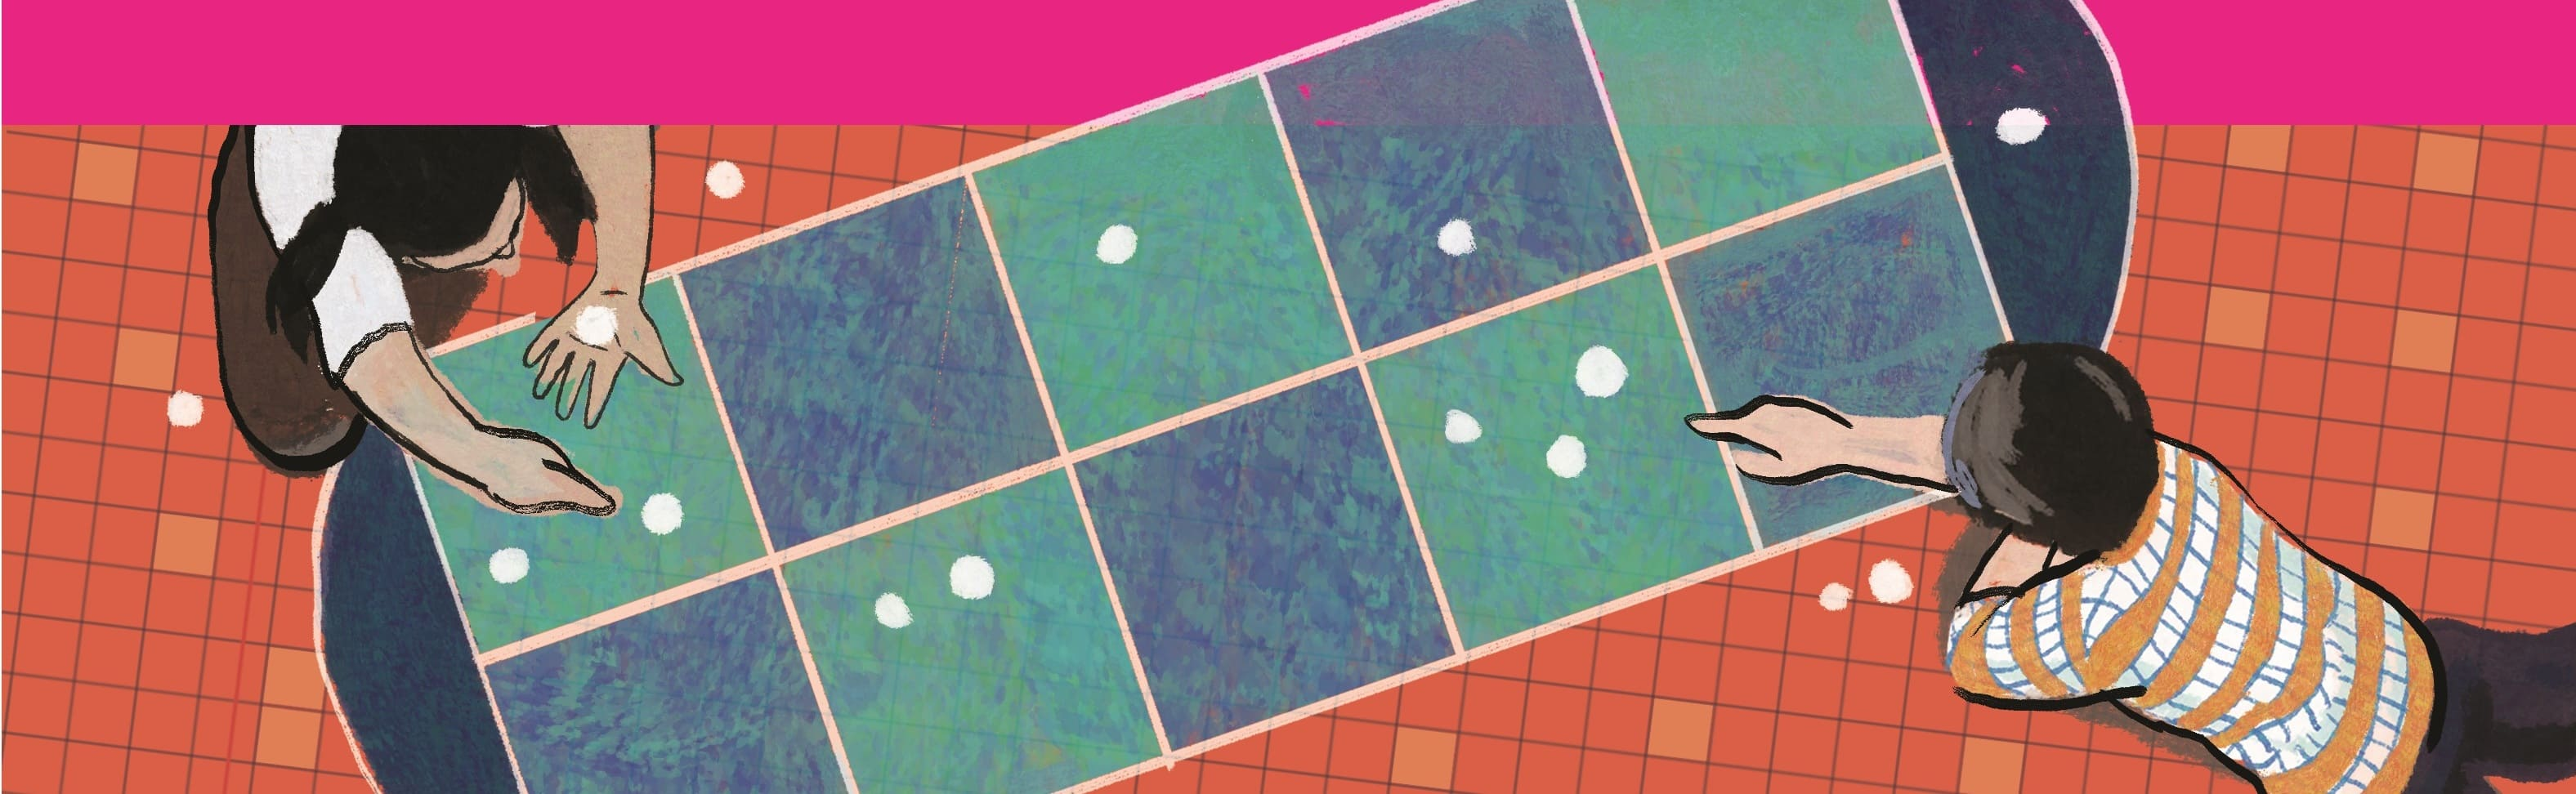
\includegraphics[width=19.3cm]{../bannertoancuabi}}}  
\AddToShipoutPicture*{\put(150,525){
\includegraphics[scale=1]{../tieudehihi.pdf}}}  
\centering
\endgroup
\vspace*{185pt} 

\begin{multicols}{2}
	$\pmb{1.}$ \textbf{\color{toancuabi}Vẽ mê cung}
	\vskip 0.1cm
	\textbf{\color{toancuabi}Cách $\pmb{1}$:}
	\vskip 0.1cm
	Dùng giấy và bút chì vẽ một hình chữ nhật có số ô vuông mỗi cạnh là lẻ, ví dụ: 
	\begin{figure}[H]
		\vspace*{-5pt}
		\centering
		\captionsetup{labelformat= empty, justification=centering}
		\begin{tikzpicture}[toancuabi, scale = 0.4, node font= \small]
			\draw (0,0) grid (15,11);
			\draw[-stealth]  (-0.5,0) -- (-0.5,11);
			\draw[-stealth]  (-0.5,11) -- (-0.5,0);
			
			\draw[-stealth]  (0,11.5) -- (15,11.5);
			\draw[-stealth]  (15,11.5) -- (0,11.5);
			\draw (-1,5.5) node [rotate = 90] {$11$ ô vuông};
			\draw (7.5,12) node  {$15$ ô vuông};
		\end{tikzpicture}
		\vspace*{-10pt}
	\end{figure}
	Sau đó, dùng bút chì tô đậm các ô vuông xen kẽ trên mỗi hàng. Những hình vuông này sẽ trở thành một phần của bức tường mê cung. 
	\begin{figure}[H]
		\vspace*{-5pt}
		\centering
		\captionsetup{labelformat= empty, justification=centering}
		\begin{tikzpicture}[toancuabi, scale = 0.4]
			\draw (0,0) grid (15,11);
			\foreach \x in {0,2,4,...,14}
				\foreach \y in {1,3,5,...,11}
					{
						\draw[fill=cackithi] (\x,\y -1) rectangle (\x + 1, \y); 
					}
		\end{tikzpicture}
		\vspace*{1pt}
	\end{figure}
	Tiếp theo, tô bóng rất nhẹ ở các ô vuông khác như hình minh họa bên dưới.
	\begin{figure}[H]
		\vspace*{-5pt}
		\centering
		\captionsetup{labelformat= empty, justification=centering}
		\begin{tikzpicture}[toancuabi, scale = 0.4]
			\foreach \x in {0,2,4,...,14}
			\foreach \y in {1,3,5,...,11}
			{
				\draw[fill=cackithi] (\x,\y -1) rectangle (\x + 1, \y); 
			}
			\foreach \x in {0,2,4,...,14}
			\foreach \y in {1,3,5,...,9}
			{
				\draw[fill=cackithi!40] (\x,\y) rectangle (\x + 1, \y+1);
			}
			\foreach \x in {1,3,5,...,13}
			\foreach \y in {1,3,5,...,11}
			{
				\draw[fill=cackithi!40] (\x,\y-1) rectangle (\x + 1, \y);
			}
		\end{tikzpicture}
		\vspace*{-5pt}
	\end{figure}
	Những hình vuông này sẽ là một phần của lối đi hoặc một phần của bức tường trong mê cung. Các ô vuông màu trắng sẽ là một phần của đường đi.
	\begin{figure}[H]
		\vspace*{-5pt}
		\centering
		\captionsetup{labelformat= empty, justification=centering}
		
\includegraphics[scale=1]{h2}
%		\caption{\small\textit{\color{}}}
		\vspace*{-10pt}
	\end{figure}
	Đã đến lúc tạo ra con đường của mê cung! Chúng ta sẽ tạo lối vào bằng cách xóa một trong những hình vuông được tô bóng mờ nhẹ để tạo một con đường quanh co dẫn đến lối ra như hình minh họa bên trên.
	\vskip 0.1cm
	Bắt đầu tạo những con đường mới từ con đường đầu tiên này, nhưng hãy làm cho chúng dẫn đến ngõ cụt để đánh lừa mọi người.
	\begin{figure}[H]
		\vspace*{-10pt}
		\centering
		\captionsetup{labelformat= empty, justification=centering}
		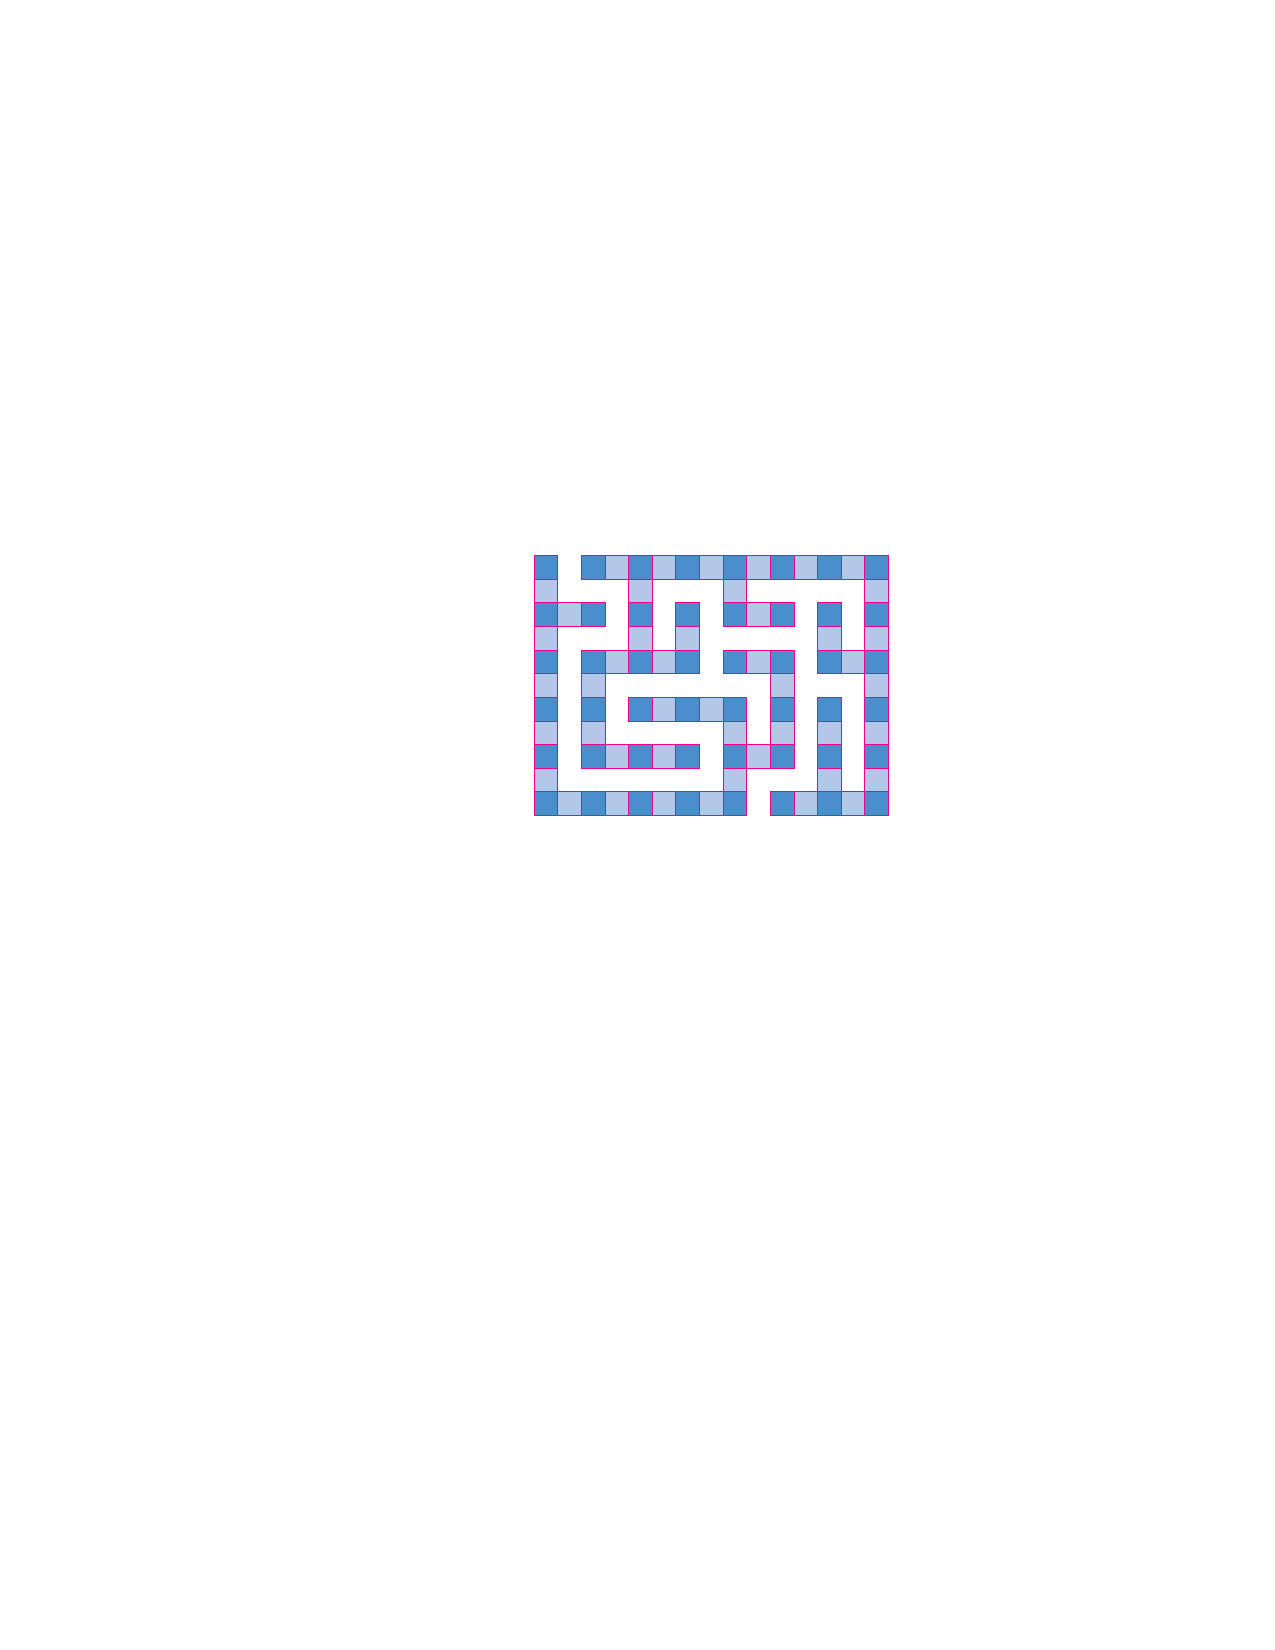
\includegraphics[scale=1]{h1}
		%		\caption{\small\textit{\color{}}}
		\vspace*{-10pt}
	\end{figure}
	Tiếp theo, tô đậm các ô vuông có bóng mờ nhẹ còn lại như hình minh họa bên dưới. Cuối cùng đánh dấu lối vào và lối ra.
	\begin{figure}[H]
		\vspace*{-10pt}
		\centering
		\captionsetup{labelformat= empty, justification=centering}
		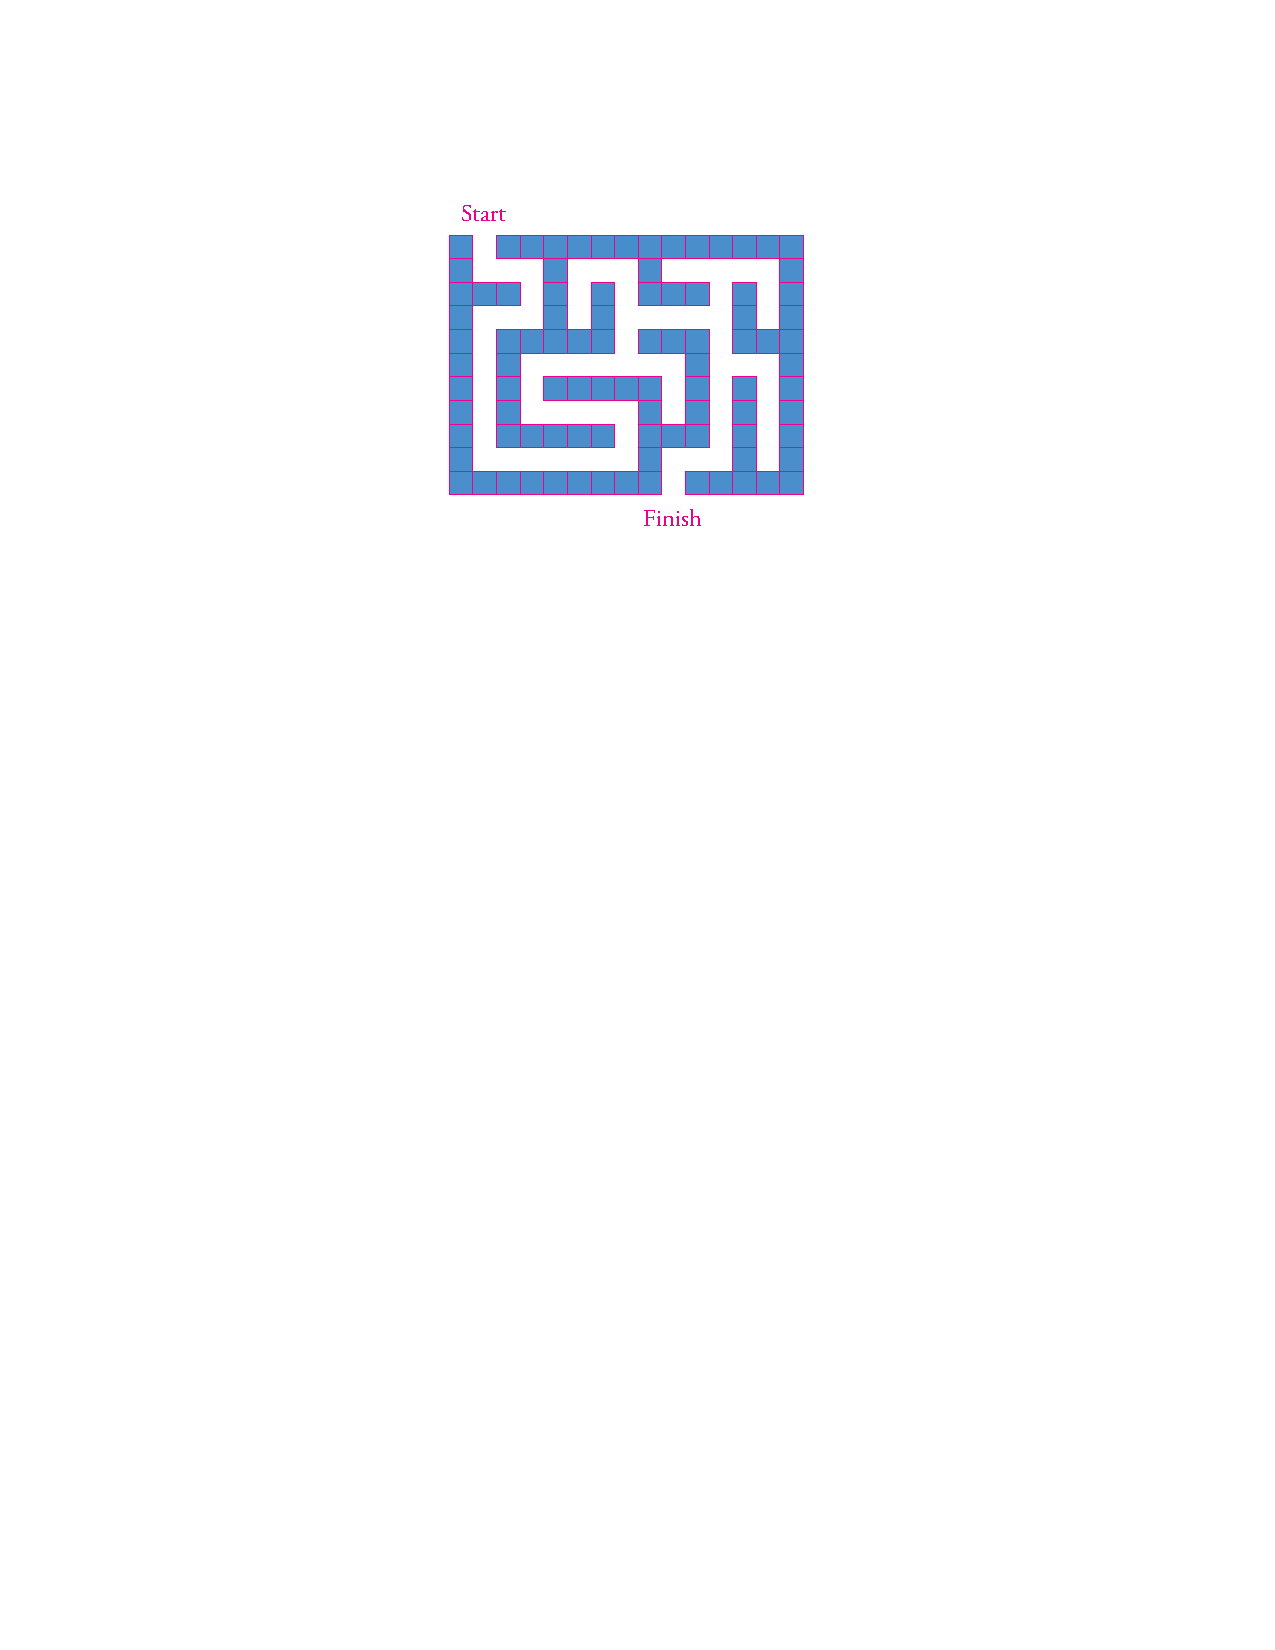
\includegraphics[scale=1]{h3}
%		\caption{\small\textit{\color{}}}
		\vspace*{-10pt}
	\end{figure}
	Vậy là mê cung đã hoàn tất! Nếu làm mê cung với quy mô càng lớn thì có thể tạo ra những mê cung khó hơn.
	\begin{figure}[H]
		\vspace*{-10pt}
		\centering
		\captionsetup{labelformat= empty, justification=centering}
		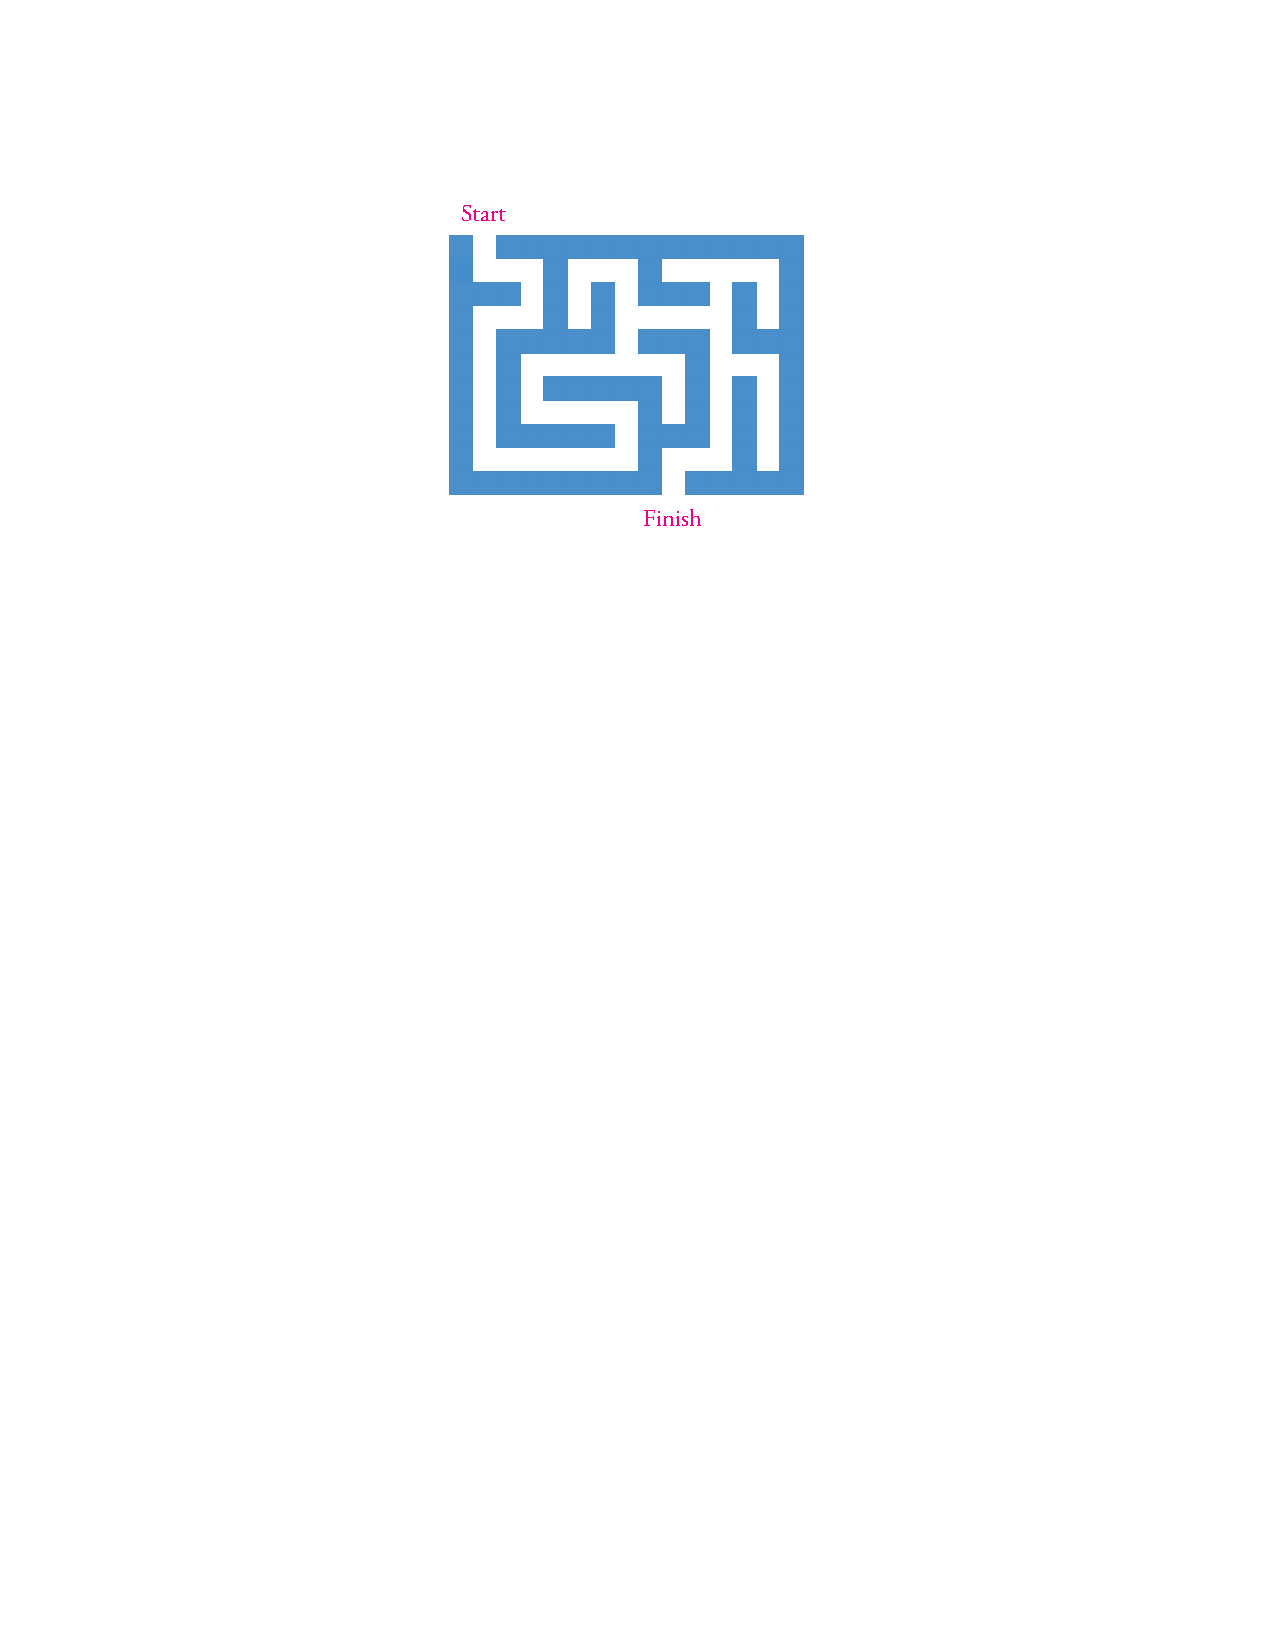
\includegraphics[scale=1]{h4}
		%		\caption{\small\textit{\color{}}}
		\vspace*{-10pt}
	\end{figure}
	\textbf{\color{toancuabi}Cách $\pmb{2:}$}
	\vskip 0.1cm  
	Bắt đầu từ giữa trang giấy, các em hãy sử dụng bút chì và thước kẻ để tạo một hàng dọc với $9$ chấm nhỏ, mỗi chấm nhỏ cách nhau $0,5$ cm.
	\begin{figure}[H]
		\vspace*{-5pt}
		\centering
		\captionsetup{labelformat= empty, justification=centering}
		\begin{tikzpicture}[toancuabi,scale=0.7]
			\draw [fill=toancuabi] (0,0) circle (2pt);
			\draw [fill=toancuabi] (0,0.5) circle (2pt);
			\draw [fill=toancuabi] (0,1) circle (2pt);
			\draw [fill=toancuabi] (0,1.5) circle (2pt);
			\draw [fill=toancuabi] (0,2) circle (2pt);
			\draw [fill=toancuabi] (0,2.5) circle (2pt);
			\draw [fill=toancuabi] (0,3) circle (2pt);
			\draw [fill=toancuabi] (0,3.5) circle (2pt);
			\draw [fill=toancuabi] (0,4) circle (2pt);
		\end{tikzpicture}
		\vspace*{-10pt}
	\end{figure}
	Sử dụng com--pa vẽ các hình bán nguyệt đồng tâm như hình minh họa bên dưới.
	\begin{figure}[H]
		\vspace*{-5pt}
		\centering
		\captionsetup{labelformat= empty, justification=centering}
		\begin{tikzpicture}[toancuabi,scale=0.7]
			\draw [fill=toancuabi] (0,0) circle (2pt);
			\draw [fill=toancuabi] (0,0.5) circle (2pt);
			\draw [fill=toancuabi] (0,1) circle (2pt);
			\draw [fill=toancuabi] (0,1.5) circle (2pt);
			\draw [fill=toancuabi] (0,2) circle (2pt);
			\draw [fill=toancuabi] (0,2.5) circle (2pt);
			\draw [fill=toancuabi] (0,3) circle (2pt);
			\draw [fill=toancuabi] (0,3.5) circle (2pt);
			\draw [fill=toancuabi] (0,4) circle (2pt);
			\begin{scope}
				\clip (-4,0) rectangle (4,4);
				\draw (0,0) circle(0.5);
				\draw (0,0) circle(1);
				\draw (0,0) circle(1.5);
				\draw (0,0) circle(2);
				\draw (0,0) circle(2.5);
				\draw (0,0) circle(3);
				\draw (0,0) circle(3.5);
				\draw (0,0) circle(4);
			\end{scope}
		\end{tikzpicture}
		\vspace*{-10pt}
	\end{figure}
	Bây giờ hãy đặt đầu nhọn của com-pa vào phía dưới bên phải của hình bán nguyệt nhỏ thứ hai.
	\begin{figure}[H]
		\vspace*{-5pt}
		\centering
		\captionsetup{labelformat= empty, justification=centering}
		\begin{tikzpicture}[toancuabi,scale=0.7]
			\draw [fill=toancuabi] (0.5,0) circle (2pt);
				\clip (-4,0) rectangle (4,4);
				\draw (0,0) circle(0.5);
				\draw (0,0) circle(1);
				\draw (0,0) circle(1.5);
				\draw (0,0) circle(2);
				\draw (0,0) circle(2.5);
				\draw (0,0) circle(3);
				\draw (0,0) circle(3.5);
				\draw (0,0) circle(4);
		\end{tikzpicture}
		\vspace*{-10pt}
	\end{figure}
	Lấy điểm này làm tâm và tạo một bộ $6$ cung tròn đồng tâm như hình minh họa bên dưới.
	\begin{figure}[H]
		\vspace*{-5pt}
		\centering
		\captionsetup{labelformat= empty, justification=centering}
		\begin{tikzpicture}[toancuabi,scale=0.7]
			\begin{scope}
				\draw [fill=toancuabi] (1,0) circle (2pt);
				\clip (-4,0) rectangle (4,4);
				\draw (0,0) circle(0.5);
				\draw (0,0) circle(1);
				\draw (0,0) circle(1.5);
				\draw (0,0) circle(2);
				\draw (0,0) circle(2.5);
				\draw (0,0) circle(3);
				\draw (0,0) circle(3.5);
				\draw (0,0) circle(4);
			\end{scope}
			\begin{scope}
				\clip (1,-3) rectangle (4,0);
				\draw (1,0) circle(0.5);
				\draw (1,0) circle(1);
				\draw (1,0) circle(1.5);
				\draw (1,0) circle(2);
				\draw (1,0) circle(2.5);
				\draw (1,0) circle(3);
			\end{scope}
		\end{tikzpicture}
		\vspace*{-10pt}
	\end{figure}
	Tiếp theo hãy đặt đầu nhọn của com--pa vào phía dưới bên trái của hình bán nguyệt nhỏ thứ ba.
	\begin{figure}[H]
		\vspace*{5pt}
		\centering
		\captionsetup{labelformat= empty, justification=centering}
		\begin{tikzpicture}[toancuabi,scale=0.7]
			\begin{scope}
				\draw [fill=toancuabi] (-1.5,0) circle (2pt);
				\clip (-4,0) rectangle (4,4);
				\draw (0,0) circle(0.5);
				\draw (0,0) circle(1);
				\draw (0,0) circle(1.5);
				\draw (0,0) circle(2);
				\draw (0,0) circle(2.5);
				\draw (0,0) circle(3);
				\draw (0,0) circle(3.5);
				\draw (0,0) circle(4);
			\end{scope}
			\begin{scope}
				\clip (1,-3) rectangle (4,0);
				\draw (1,0) circle(0.5);
				\draw (1,0) circle(1);
				\draw (1,0) circle(1.5);
				\draw (1,0) circle(2);
				\draw (1,0) circle(2.5);
				\draw (1,0) circle(3);
			\end{scope}
		\end{tikzpicture}
		\vspace*{-5pt}
	\end{figure}
	Lần này tạo một bộ gồm $5$ cung tròn đồng tâm như hình minh họa bên dưới.
	\begin{figure}[H]
		\vspace*{-5pt}
		\centering
		\captionsetup{labelformat= empty, justification=centering}
		\begin{tikzpicture}[toancuabi,scale=0.7]
			\begin{scope}
				\draw [fill=toancuabi] (-1.5,0) circle (2pt);
				\clip (-4,0) rectangle (4,4);
				\draw (0,0) circle(0.5);
				\draw (0,0) circle(1);
				\draw (0,0) circle(1.5);
				\draw (0,0) circle(2);
				\draw (0,0) circle(2.5);
				\draw (0,0) circle(3);
				\draw (0,0) circle(3.5);
				\draw (0,0) circle(4);
			\end{scope}
			\begin{scope}
				\clip (1,-3) rectangle (4,0);
				\draw (1,0) circle(0.5);
				\draw (1,0) circle(1);
				\draw (1,0) circle(1.5);
				\draw (1,0) circle(2);
				\draw (1,0) circle(2.5);
				\draw (1,0) circle(3);
			\end{scope}
			\begin{scope}
				\clip (-1.5,0) rectangle (-4,-4);
				\draw (-1.5,0) circle(0.5);
				\draw (-1.5,0) circle(1);
				\draw (-1.5,0) circle(1.5);
				\draw (-1.5,0) circle(2);
				\draw (-1.5,0) circle(2.5);
			\end{scope}
		\end{tikzpicture}
		\vspace*{-10pt}
	\end{figure}
	Vẽ một đường thẳng nằm ngang để nối hai cung tròn như hình minh họa bên dưới.
	\begin{figure}[H]
		\vspace*{-5pt}
		\centering
		\captionsetup{labelformat= empty, justification=centering}
		\begin{tikzpicture}[toancuabi,scale=0.7]
			\begin{scope}
%				\draw [fill=toancuabi] (-1.5,0) circle (2pt);
				\clip (-4,0) rectangle (4,4);
				\draw (0,0) circle(0.5);
				\draw (0,0) circle(1);
				\draw (0,0) circle(1.5);
				\draw (0,0) circle(2);
				\draw (0,0) circle(2.5);
				\draw (0,0) circle(3);
				\draw (0,0) circle(3.5);
				\draw (0,0) circle(4);
			\end{scope}
			\begin{scope}
				\clip (1,-3) rectangle (4,0);
				\draw (1,0) circle(0.5);
				\draw (1,0) circle(1);
				\draw (1,0) circle(1.5);
				\draw (1,0) circle(2);
				\draw (1,0) circle(2.5);
				\draw (1,0) circle(3);
			\end{scope}
			\begin{scope}
				\clip (-1.5,0) rectangle (-4,-4);
				\draw (-1.5,0) circle(0.5);
				\draw (-1.5,0) circle(1);
				\draw (-1.5,0) circle(1.5);
				\draw (-1.5,0) circle(2);
				\draw (-1.5,0) circle(2.5);
			\end{scope}
			\draw (-1.5,-1) -- (1,-1);
		\end{tikzpicture}
		\vspace*{-10pt}
	\end{figure}
	Tiếp theo vẽ một đường thẳng đứng xuống từ phía bên trái của hình bán nguyệt nhỏ nhất.
	\begin{figure}[H]
		\vspace*{5pt}
		\centering
		\captionsetup{labelformat= empty, justification=centering}
		\begin{tikzpicture}[toancuabi,scale=0.7]
			\begin{scope}
				\clip (-4,0) rectangle (4,4);
				\draw (0,0) circle(0.5);
				\draw (0,0) circle(1);
				\draw (0,0) circle(1.5);
				\draw (0,0) circle(2);
				\draw (0,0) circle(2.5);
				\draw (0,0) circle(3);
				\draw (0,0) circle(3.5);
				\draw (0,0) circle(4);
			\end{scope}
			\begin{scope}
				\clip (1,-3) rectangle (4,0);
				\draw (1,0) circle(0.5);
				\draw (1,0) circle(1);
				\draw (1,0) circle(1.5);
				\draw (1,0) circle(2);
				\draw (1,0) circle(2.5);
				\draw (1,0) circle(3);
			\end{scope}
			\begin{scope}
				\clip (-1.5,0) rectangle (-4,-4);
				\draw (-1.5,0) circle(0.5);
				\draw (-1.5,0) circle(1);
				\draw (-1.5,0) circle(1.5);
				\draw (-1.5,0) circle(2);
				\draw (-1.5,0) circle(2.5);
			\end{scope}
			\draw (-1.5,-1) -- (1,-1);
			\draw (-0.5,0) -- (-0.5,-2);
		\end{tikzpicture}
		\vspace*{-10pt}
	\end{figure}
	Cẩn thận uốn cong đường thẳng này để nó chạm vào cạnh của cung tròn lớn nhất ở phía dưới bên phải.
	\begin{figure}[H]
		\vspace*{-5pt}
		\centering
		\captionsetup{labelformat= empty, justification=centering}
		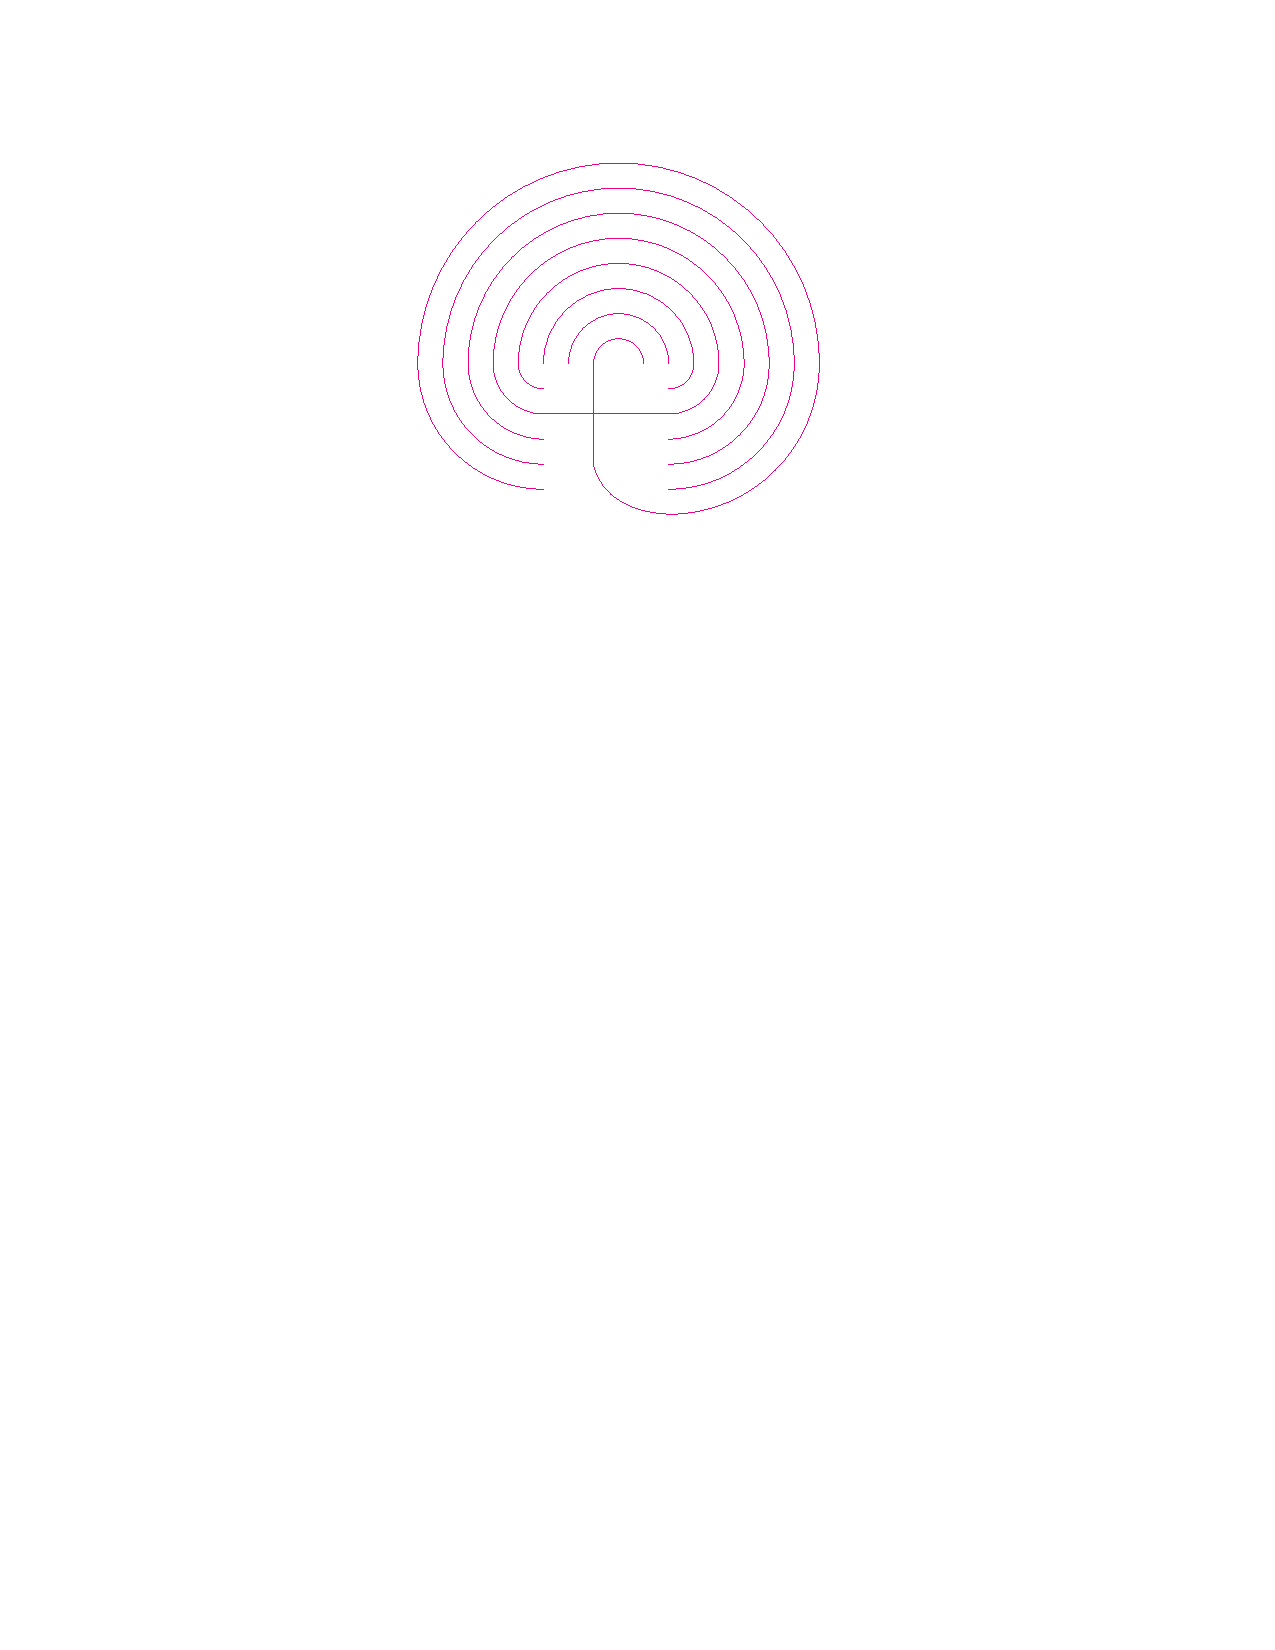
\includegraphics[scale =0.8]{h5}
%		\caption{\small\textit{\color{}}}
		\vspace*{-10pt}
	\end{figure}
	Cuối cùng, hoàn thiện phần còn lại của mê cung như hình minh họa bên dưới.
	\begin{figure}[H]
		\vspace*{-5pt}
		\centering
		\captionsetup{labelformat= empty, justification=centering}
		
\includegraphics[scale =0.8]{h6}
%		\caption{\small\textit{\color{}}}
		\vspace*{-10pt}
	\end{figure}
	\textbf{\color{toancuabi}Tài liệu tham khảo}
	\vskip 0.1cm
	\url{https://www.artfulmaths.com/mathemati}\\
	\url{cal-art-lessons.html}
\end{multicols}
%\newpage
%\begingroup
%\AddToShipoutPicture*{\put(60,628){
\includegraphics[scale=1]{../tieude1.pdf}}} 
%\centering
%\endgroup
%\vspace*{70pt}
%
%\begin{multicols}{2}
%	Tiếp tục với nội dung về đề thi tuyển sinh vào Câu lạc bộ Unicorn Math Circle, trong số này, tạp chí Pi giới thiệu đến bạn đọc bài thi dành cho các bạn học sinh lớp $7$. Thời gian đề xuất làm bài là $90$ phút. 
%	\vskip 0.1cm
%	\textbf{\color{toancuabi}\color{toancuabi}Bài $\pmb1$.} Tìm một số có $3$ chữ số mà khi tăng chữ số hàng trăm lên $3$ đơn vị, chữ số hàng chục lên $2$ đơn vị và chữ số hàng đơn vị lên $1$ đơn vị thì ta nhận được số mới gấp $4$ lần số ban đầu.
%	\vskip 0.1cm
%	\textbf{\color{toancuabi}\color{toancuabi}Bài $\pmb2$.} Trên bảng có viết số $798798798798$. Bạn cần xóa đi một hoặc vài chữ số để kết quả nhận được là một số chia hết cho $9$. Hỏi số lớn nhất mà bạn có thể nhận được là bao nhiêu?
%	\vskip 0.1cm
%	\textbf{\color{toancuabi}\color{toancuabi}Bài $\pmb3$.} Năm học $2022-2023$ là một năm học đặc biệt: không thể đổi chỗ các chữ số của số $2022$ để có một số nhỏ hơn $2022$ và số $2023$ cũng như vậy. (Các số không được bắt đầu bằng chữ số $0$). Hỏi năm học nào gần nhất trước đó cũng đặc biệt như vậy?
%	\vskip 0.1cm
%	\textbf{\color{toancuabi}\color{toancuabi}Bài $\pmb4$.} Hãy đưa ra ví dụ $5$ số hữu tỷ phân biệt nằm giữa $\dfrac{1}{2022}$ và $\dfrac{1}{2023}.$
%	\vskip 0.1cm
%	\textbf{\color{toancuabi}\color{toancuabi}Bài $\pmb5$.} Có bao nhiêu số có $3$ chữ số khác nhau, chia hết cho $11$, được tạo thành từ các chữ số $1,3,5,7,9$?
%	\vskip 0.1cm
%	\textbf{\color{toancuabi}\color{toancuabi}Bài $\pmb6$.} Tìm số tự nhiên $n$  nhỏ nhất sao cho $(n + 1)( n + 2)( n + 3)( n + 4)$ chia hết cho $1000$.
%	\vskip 0.1cm
%	\textbf{\color{toancuabi}\color{toancuabi}Bài $\pmb7$.} Tom viết tất cả các số tự nhiên sao cho tích các chữ số của mỗi số bằng $2016$. Jerry chọn số nhỏ nhất trong chúng. Hỏi Jerry đã chọn số nào?
%	\vskip 0.1cm
%	\textbf{\color{toancuabi}\color{toancuabi}Bài $\pmb8$.} Trong một giải đấu thể dục dụng cụ, mỗi vận động viên được hội đồng giám khảo gồm $7$ người chấm điểm. Mỗi giám khảo cho điểm là một số tự nhiên từ $1$ đến $10$. Sau đó, theo quy định, trong số các điểm mà $7$ giám khảo chấm thì một điểm cao nhất và một điểm thấp nhất sẽ bị loại bỏ (nếu có nhiều điểm cao nhất hoặc thấp nhất bằng nhau thì chỉ loại bỏ một trong số đó) và điểm số chính thức của vận động viên là tổng của $5$ điểm còn lại. Sau một màn trình diễn, một vận động viên được $7$ giám khảo cho tổng số điểm bằng $37$. Hỏi điểm số chính thức của vận động viên đó cao nhất có thể bằng bao nhiêu?
%	\vskip 0.1cm
%	\textbf{\color{toancuabi}\color{toancuabi}Bài $\pmb{9}$.} Nêu một cách điền các số $1$ và $-1$ vào các ô của một bảng $5\times 6$, mỗi ô một số, sao cho nếu lấy tổng của các số trên các hàng và các cột của bảng thì ta nhận được $11$ số khác nhau.
%	\vskip 0.1cm
%	\textbf{\color{toancuabi}\color{toancuabi}Bài $\pmb{10}$.} Trên một hòn đảo nhỏ có $40$ cư dân gồm hai loại người: người Dối trá, luôn luôn nói dối và người Khôn ngoan, khi thì nói thật lúc lại nói dối. Một hôm tất cả các cư dân ngồi họp quanh một bàn tròn và mỗi người đều nói ``Ngồi sát bên cạnh tôi là một người Dối trá và một người Khôn ngoan". Biết rằng lần đó có đúng $3$ người Khôn ngoan nói dối. Hỏi trên đảo có tất cả bao nhiêu người Dối trá.
%	\vskip 0.1cm
%	\textbf{\color{toancuabi}\color{toancuabi}Đáp án}
%	\vskip 0.1cm
%	\textbf{\color{toancuabi}\color{toancuabi}Bài $\pmb{1}$.} $107$.
%	\vskip 0.05cm
%	\textbf{\color{toancuabi}\color{toancuabi}Bài $\pmb{2}$.} $9879879879$.
%	\vskip 0.1cm
%	\textbf{\color{toancuabi}\color{toancuabi}Bài $\pmb{3}$.} $2008-2009$.
%	\vskip 0.1cm
%	\textbf{\color{toancuabi}\color{toancuabi}Bài $\pmb{4}$.} Bài toán có nhiều đáp án, một đáp án mẫu là: $\dfrac{10}{20221}; \dfrac{10}{20222}; \dfrac{10}{20223}; \dfrac{10}{20224}; \dfrac{10}{20225}.$
%	\vskip 0.1cm
%	\textbf{\color{toancuabi}\color{toancuabi}Bài $\pmb{5}$.} $8$.
%	\vskip 0.1cm
%	\textbf{\color{toancuabi}\color{toancuabi}Bài $\pmb{6}$.} $121$.
%	\vskip 0.1cm
%	\textbf{\color{toancuabi}\color{toancuabi}Bài $\pmb{7}$.} $4789$.
%	\vskip 0.1cm
%	\textbf{\color{toancuabi}\color{toancuabi}Bài $\pmb{8}$.} \textit{Lời giải.}
%	Một mặt, điếm số thấp nhất không ít hơn $1$. Mặt khác, do tổng điểm của $7$ giám khảo bằng $37$ nên có một giám khảo cho điểm từ $6$ trở lên (nếu không, tổng số điểm của $7$ giám khảo không vượt quá $7\times 5=35$). Như vậy, tổng điểm của giám khảo cho thấp nhất và cao nhất không ít hơn $1+ 6=7$. Chính vì vậy, điểm chính thức của vận động viên cao nhất là $37-7=30$. Đảo lại, nếu các giám khảo cho điểm là $1, 6, 6, 6, 6, 6, 6$ thì điểm chính thức của vận động viên đúng bằng $30$.
%	Đáp số $30$.
%	\vskip 0.1cm
%	\textbf{\color{toancuabi}\color{toancuabi}Bài $\pmb{9}$.} \textit{Lời giải.} Một ví dụ
%	\begin{center}
%		\begin{tikzpicture}
%			\draw (0,0) grid (6, 5);
%			\foreach \y in {0,...,4} \node at (0.5,\y+0.5){$-1$};
%			\foreach \y in {1,...,4} \node at (1.5,\y+0.5){$-1$};
%			\foreach \x in {1,...,5} \node at (\x+ 0.5,0.5){$1$};
%			\foreach \x in {2,...,4} \node at (\x+ 0.5,4.5){$-1$};
%			\foreach \x in {2,...,5} \node at (\x+ 0.5,3.5){$1$};
%			\foreach \x in {3,...,5} \node at (\x+ 0.5,2.5){$1$};
%			\foreach \x in {4,...,5} \node at (\x+ 0.5,1.5){$1$};
%			\foreach \x in {2,...,3} \node at (\x+ 0.5,1.5){$-1$};
%			\node at (2.5,2.5){$-1$};
%			\node at (5.5,4.5){$1$};
%			\node at (0.5,-0.5){$-5$};
%			\node at (1.5,-0.5){$-3$};
%			\node at (2.5,-0.5){$-1$};
%			\node at (3.5,-0.5){$1$};
%			\node at (4.5,-0.5){$3$};
%			\node at (5.5,-0.5){$5$};
%			\node at (6.5,0.5){$4$};
%			\node at (6.5,1.5){$-2$};
%			\node at (6.5,2.5){$0$};
%			\node at (6.5,3.5){$2$};
%			\node at (6.5,4.5){$-4$};
%		\end{tikzpicture}
%	\end{center}
%\textbf{\color{toancuabi}\color{toancuabi}Bài $\pmb{10}$.} \textit{Lời giải.} Nhận xét rằng nếu có $2$ người Dối trá ngồi cạnh nhau thì bên cạnh những người này phải đều là những người Dối trá. Và cứ tiếp tục như vậy thì không bao giờ xuất hiện người Khôn Ngoan, điều này là vô lý. Do đó giữa $2$ người Dối trá luôn có ít nhất $1$ người Khôn ngoan.
%\vskip 0.1cm
%Ta thấy rằng chỉ có đúng $2$ trường hợp mà một người Khôn Ngoan nói dối:
%\vskip 0.1cm
%\textit{Trường hợp} $1$: Nếu giữa hai người Dối trá có đúng $1$ người Khôn ngoan, thì người này đã nói dối;
%\vskip 0.1cm
%\textit{Trường hợp} $2$: Cũng như vậy, nếu giữa hai người Dối trá có đúng $k \ge 2$ người Khôn ngoan thì sẽ có đúng $k - 2$ người Khôn Ngoan ở chính giữa đã nói dối.
%\vskip 0.1cm
%Gọi số người Khôn ngoan đã nói dối trong TH$1$ là $a$ và TH$2$ là $b$ thì $a + b = 3$. Hơn nữa nếu ta bỏ đi những người loại $b$ thì trong số các cặp $2$ người Dối trá liên tiếp sẽ có đúng $a$ cặp có $1$ người Khôn ngoan, các cặp còn lại có đúng $2$ người Khôn ngoan. Do đó ta suy ra: $40 − b + a$ chia hết cho $3$. Chỉ có thể xảy ra điều này nếu $a = 1, b = 2$. Từ đây dễ dàng suy ra có $13$ người Dối trá.
%\end{multicols}
%\newpage
%\begingroup
%\AddToShipoutPicture*{\put(110,675){
\includegraphics[scale=1]{../tieude.pdf}}}  
%\centering
%\endgroup
%\vspace*{25pt} 
%\begin{multicols}{2}
%	Thám tử Xuân Phong cùng thanh tra Lê Kính được bên cảnh sát mời tới thẩm tra các đối tượng vừa bị bắt giữ tại khu tạm giam. Theo ý kiến đề xuất của Xuân Phong, Lê Kính cho mời $20$ đối tượng từ hai băng cướp có tên là Mèo Rừng và Báo Hoa vào phòng và phát riêng cho mỗi đối tượng một câu hỏi. Có tất cả $20$ câu hỏi được in ra trên các tấm bìa gồm hai màu xanh và hồng. Không đối tượng nào nhìn thấy màu tấm bìa mà đối tượng khác được phát. Qua bên cảnh sát thuật lại, các tên cướp từ băng Mèo Rừng luôn nói thật, còn các tên cướp từ băng Báo Hoa luôn nói dối. Sau khi đã được phát các câu hỏi, tất cả các đối tượng đều tuyên bố ``Tôi đã nhận được câu hỏi in trên tấm bìa màu xanh". Sau đó, các câu hỏi được thu lại, tráo đều lên và lại được phát lần thứ hai cho các đối tượng. Lần này thì chỉ có một nửa số các đối tượng được triệu tập tuyên bố ``Trong lần phát  thứ hai này tôi đã nhận được câu hỏi in trên tấm bìa màu xanh", còn tất cả các đối tượng còn lại đều tuyên bố ``Trong lần phát  thứ hai này tôi đã nhận được câu hỏi in trên tấm bìa màu hồng". 
%	\vskip 0.1cm
%	Em hãy giúp thám tử Xuân Phong tìm ra số các đối tượng đến từ băng Mèo Rừng đã nhận được câu hỏi in trên tấm bìa màu hồng trong lần phát câu hỏi thứ hai nhé.
%	\begin{figure}[H]
%		\vspace*{-5pt}
%		\centering
%		\captionsetup{labelformat= empty, justification=centering}
%		
\includegraphics[width= 1\linewidth]{XuanPhong}
%%		\caption{\small\textit{\color{}.}}
%		\vspace*{-5pt}
%	\end{figure}
%\end{multicols}
%\vspace*{-10pt}
%{\color{toancuabi}\rule{1\linewidth}{0.1pt}}
%\begingroup
%\AddToShipoutPicture*{\put(112,298){
\includegraphics[scale=1]{../tieude11.pdf}}} 
%\centering
%\endgroup
%\vspace*{50pt}
%
%\begin{multicols}{2}
%	$\pmb{1.}$ 	Hai đoàn tàu xuất phát cùng một thời điểm trên một tuyến đường sắt, một tàu đi từ $A$ tới $B$ với tốc độ $80$ km/h, tàu còn lại đi từ $B$ tới $A$ với vận tốc $70$ km/h. Hỏi trước khi gặp nhau một giờ hai tàu cách nhau bao nhiêu km, cho biết quãng đường từ $A$ tới $B$ dài ít nhất là $350$ km.
%	\begin{figure}[H]
%			\centering
%			\vspace*{-5pt}
%			\captionsetup{labelformat= empty, justification=centering}
%			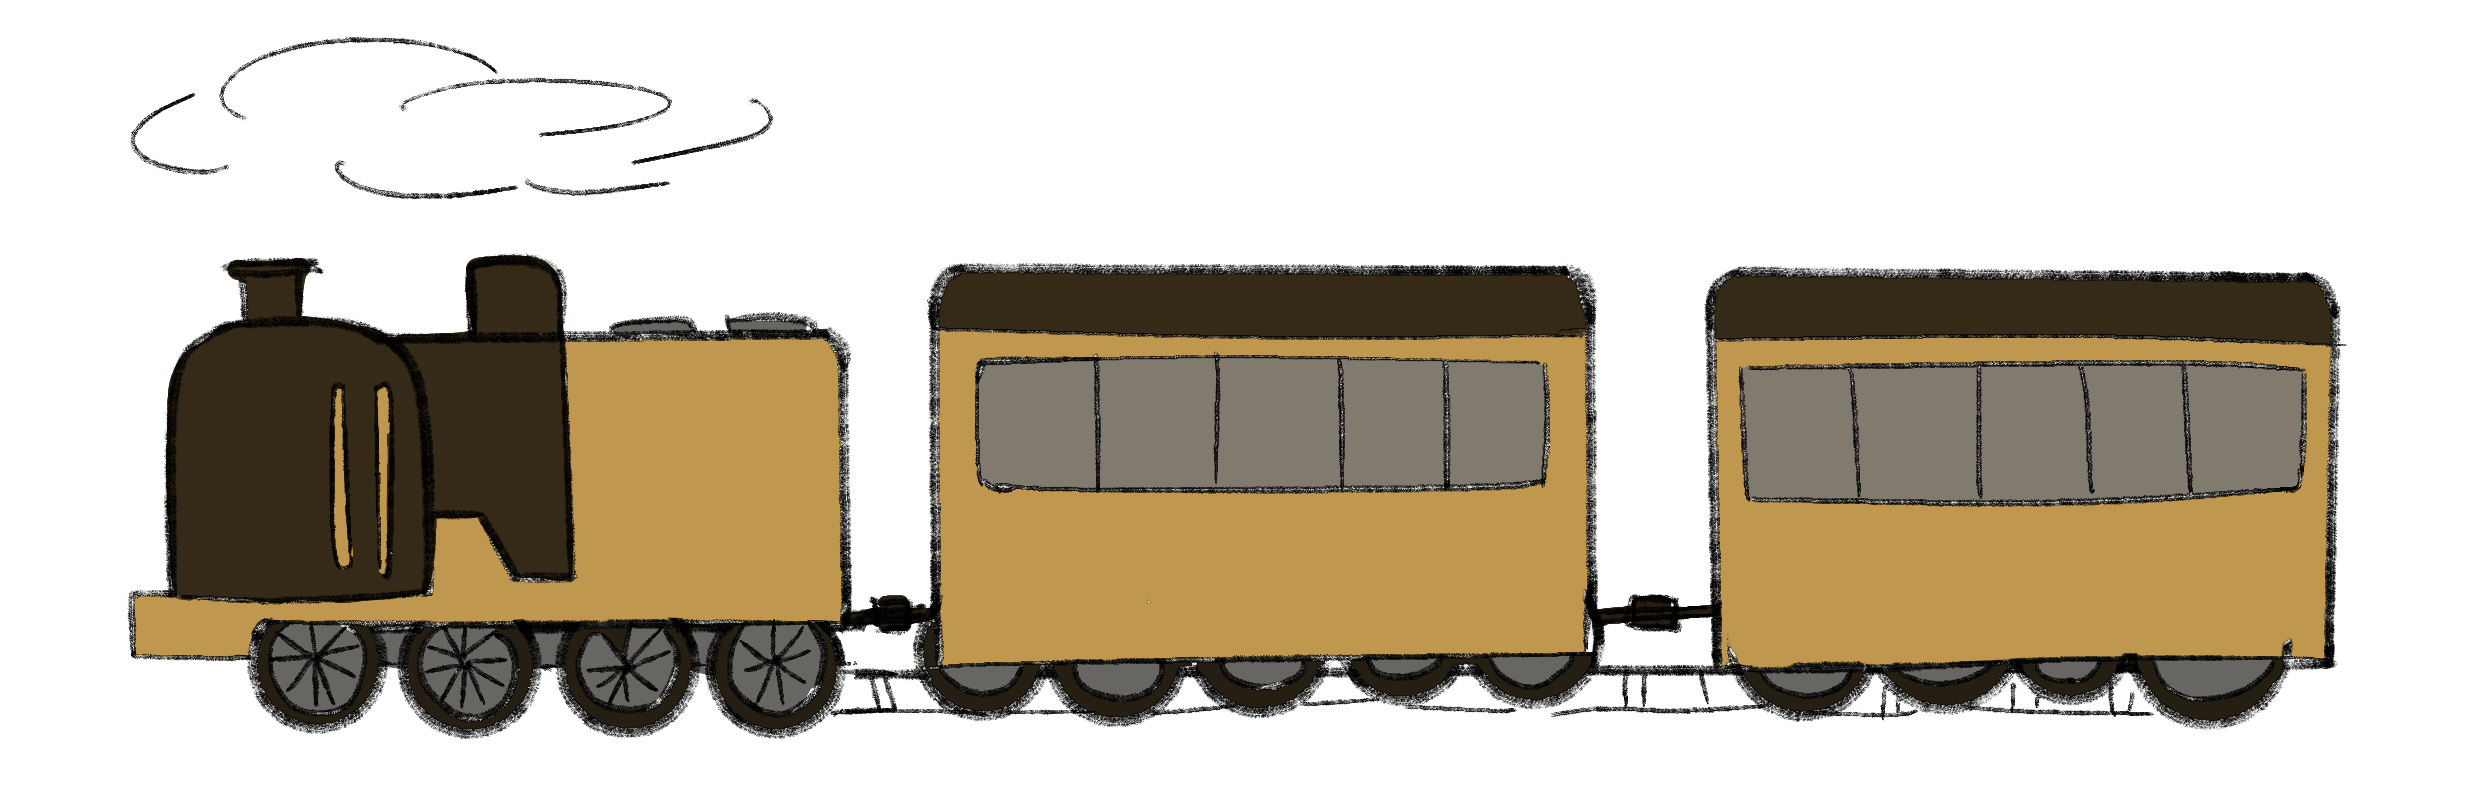
\includegraphics[width=1\linewidth]{Bai1}
%			\vspace*{-15pt}
%		\end{figure}
%	$\pmb{2.}$ Anh Sơn xuất phát từ chân dốc và đi lên dốc với tốc độ $2.5$ km/h. Lên đến đỉnh dốc, anh đi xuống với tốc độ là $5$ km/h. Tổng thời gian đi và về của anh Sơn là $6$h. Em hãy tính quãng đường từ chân dốc lên đỉnh dốc. 	
%	\begin{figure}[H]
%			\centering
%			\vspace*{-5pt}
%			\captionsetup{labelformat= empty, justification=centering}
%			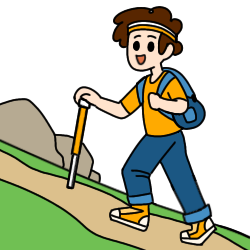
\includegraphics[width=0.72\linewidth]{Bai2}
%%			\vspace*{-5pt}
%		\end{figure}
%	$\pmb{3.}$ Tí đi mua bánh rán hết $45$ ngàn đồng. Bánh rán cỡ to giá $7$ ngàn đồng/chiếc, cỡ nhỏ giá $5$ ngàn đồng/chiếc. Tí đã ăn luôn một chiếc bánh to sau khi mua, hỏi Tí còn lại mấy chiếc bánh rán?	
%	\begin{figure}[H]
%			\centering
%			\vspace*{-5pt}
%			\captionsetup{labelformat= empty, justification=centering}
%			\includegraphics[width=0.85\linewidth]{bai3}
%			\vspace*{-15pt}
%		\end{figure}
%	$\pmb{4.}$ Bác Tâm có $100$ quả trứng gà. Bác bỏ chúng vào $5$ chiếc rổ. Tổng số trứng trong rổ thứ nhất và thứ hai là $52$, số trứng trong rổ thứ hai và thứ ba là $43$, trong rổ thứ ba và thứ tư là $34$, tổng số trứng trong hai rổ cuối cùng là $30$.  Hỏi số trứng trong mỗi rổ là bao nhiêu?	
%	\begin{figure}[H]
%			\centering
%			\vspace*{-5pt}
%			\captionsetup{labelformat= empty, justification=centering}
%			\includegraphics[width=0.9\linewidth]{bai4}
%			\vspace*{-10pt}
%	\end{figure}
%	$\pmb{5.}$ Có $3$ đĩa đựng những quả táo, trong đó một đĩa có $11$ quả, $1$ đĩa có $7$ quả và đĩa còn lại có $6$ quả táo. Người ta muốn chuyển chỗ những quả táo giữa các đĩa sao cho số táo trên ba đĩa bằng nhau với điều kiện mỗi lần thêm táo vào một đĩa, số táo thêm vào phải bằng số táo hiện có trên đĩa đó và tất cả những quả táo được thêm vào lấy ra từ chỉ một đĩa trong hai đĩa còn lại. Em hãy cho biết có thể thực hiện với $3$ lần chuyển chỗ những quả táo hay không?	
%	\begin{figure}[H]
%			\centering
%			\vspace*{-5pt}
%			\captionsetup{labelformat= empty, justification=centering}
%			\includegraphics[width=1\linewidth]{bai5}
%			\vspace*{-20pt}
%		\end{figure}
%	$\pmb{6.}$ Ban đầu bốn bạn An, Bách, Công, Dũng mỗi người có một số viên bi nhất định trong đó Công có nhiều hơn Dũng $10$ viên bi. Nếu Công cho Bách $\frac{1}{4}$  số bi của mình,  An lấy $\frac{1}{3}$ số bi của An cho Bách, tiếp đến Bách cho Công $\frac{1}{4}$ số bi Bách hiện có, rồi Công lại cho $\frac{1}{5}$ số bi của mình đang có cho Dũng và cuối cùng Bách lấy $\frac{1}{4}$ số bi chia đều cho $3$ bạn còn lại thì bốn bạn có số viên bi bằng nhau. Ban đầu mỗi bạn có bao nhiêu viên bi?
%	\begin{figure}[H]
%		\centering
%		\vspace*{-10pt}
%		\captionsetup{labelformat= empty, justification=centering}
%		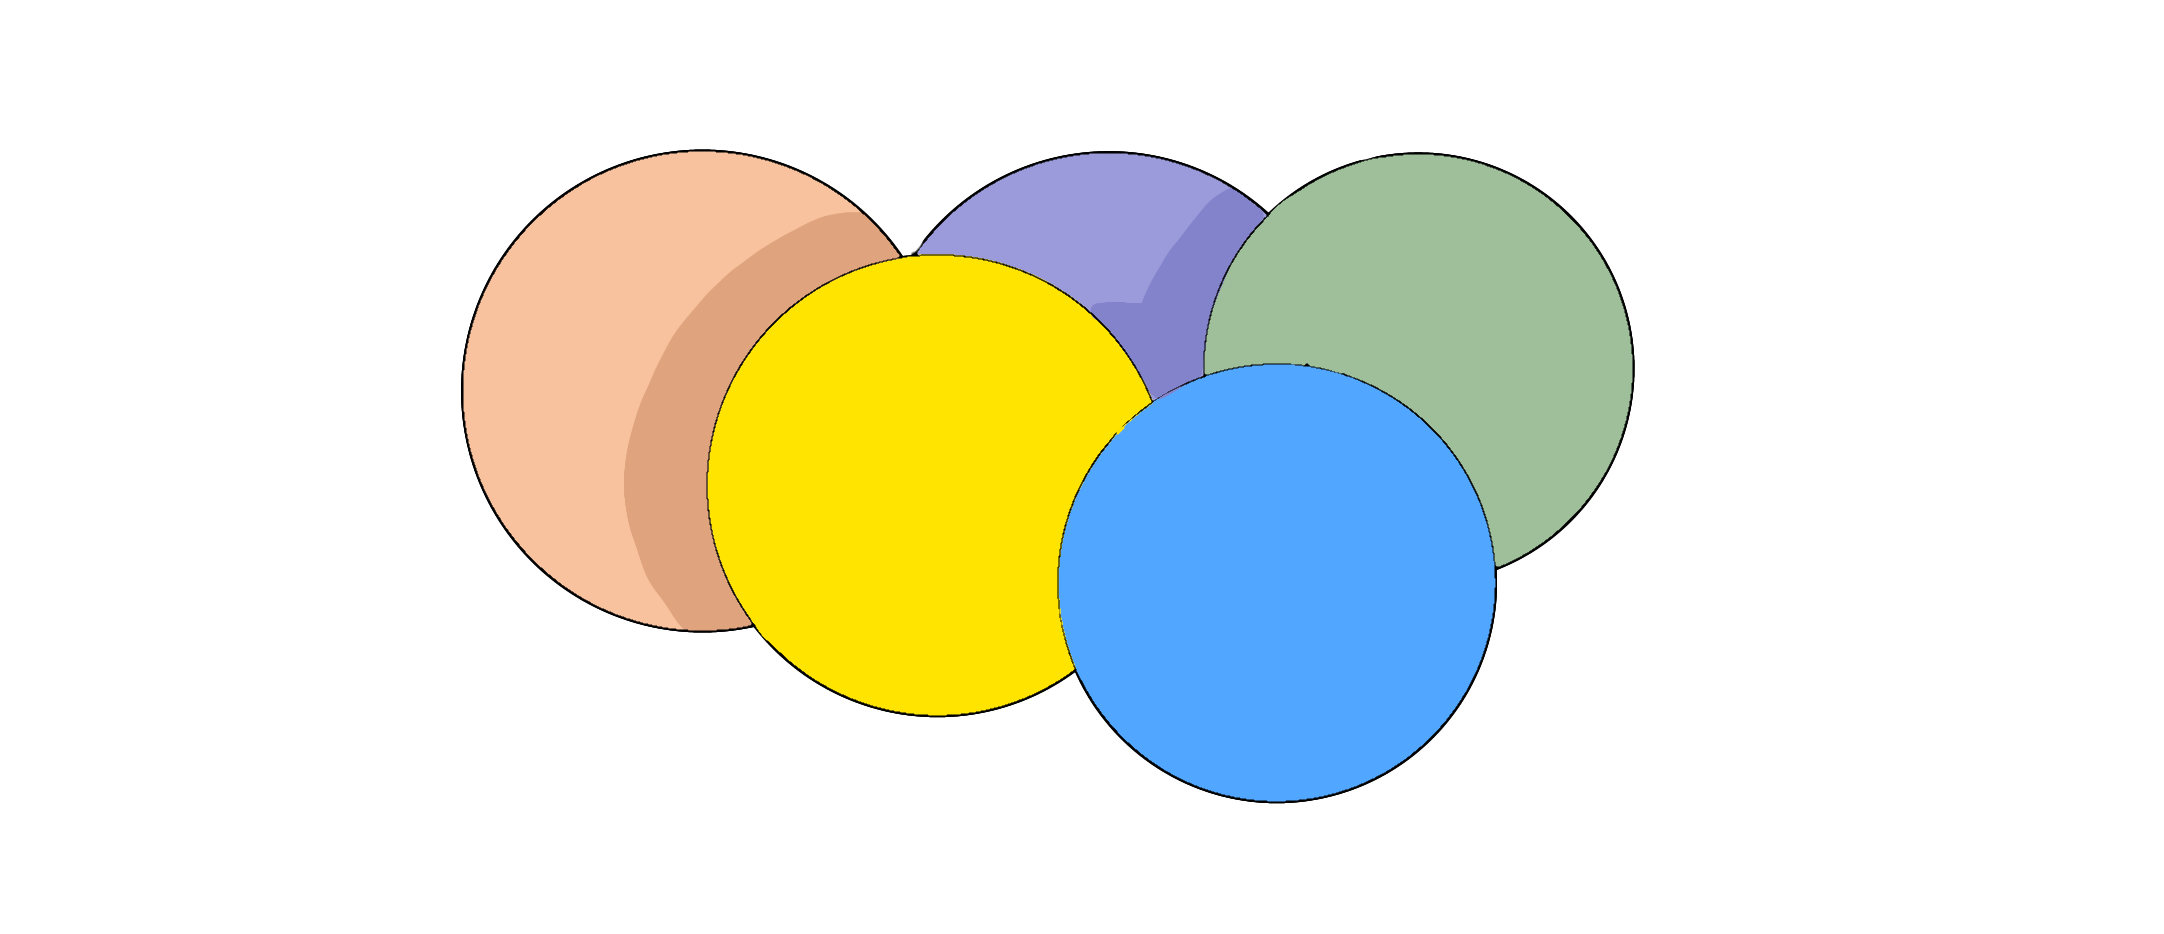
\includegraphics[width=1\linewidth]{Bai6}
%		\vspace*{-10pt}
%	\end{figure}
%\end{multicols}
%\newpage
%\begingroup
%\AddToShipoutPicture*{\put(114,640){
\includegraphics[scale=1]{../tieude2.pdf}}} 
%\centering
%\endgroup
%\vspace*{65pt}
%
%\begin{multicols}{2}
%	$\pmb{1.}$ Tuấn và Tú cùng tham gia một giải thi đấu cờ vua cùng các bạn học sinh khác trong trường. Hai bạn tổng cộng ghi được $6{.}5$ điểm, trong khi tất cả các bạn học sinh còn lại đều ghi được số điểm bằng nhau. Hỏi có tất cả bao nhiêu học sinh tham gia giải cờ vua đó? (Biết rằng trong giải thi đấu, mỗi người tham gia thi đấu đúng một ván với mỗi người còn lại, ghi được $1$ điểm sau mỗi trận thắng, $0{.}5$ điểm sau mỗi trận hoà và $0$ điểm sau mỗi trận thua).
%	\begin{figure}[H]
%		\centering
%		\vspace*{-5pt}
%		\captionsetup{labelformat= empty, justification=centering}
%		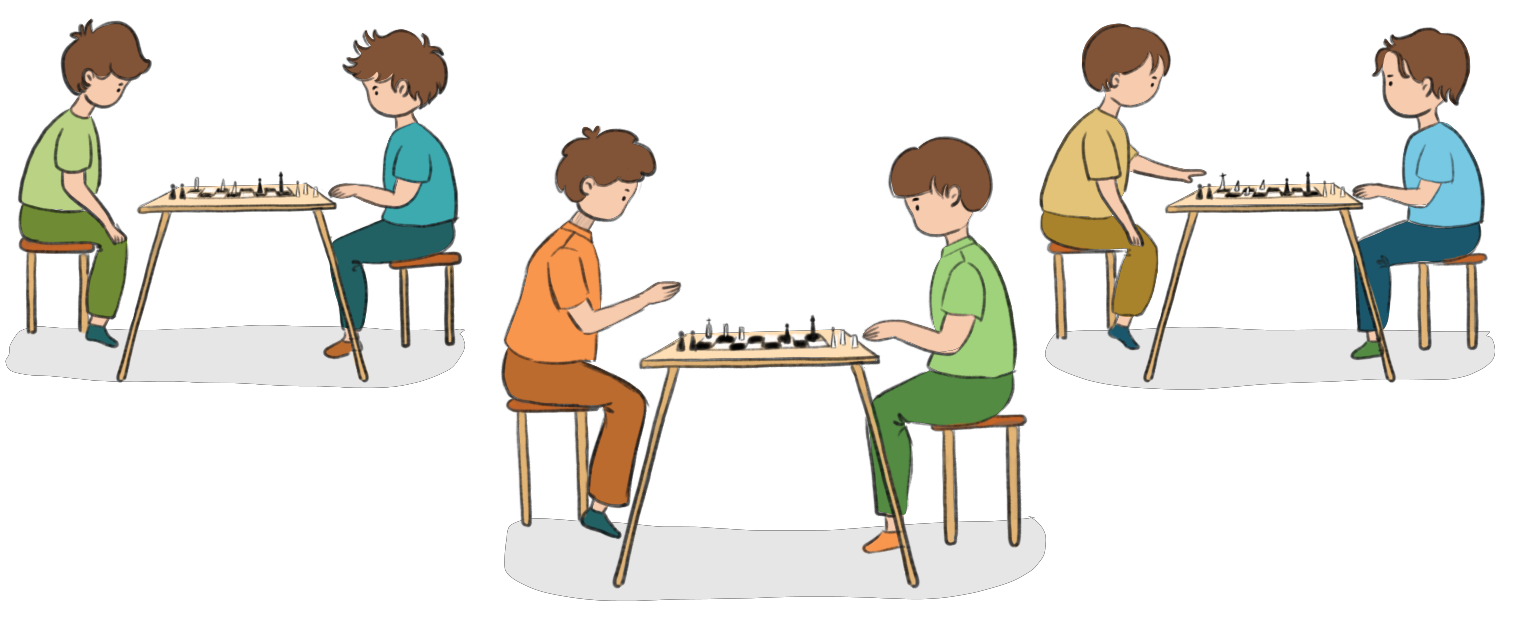
\includegraphics[width=1\linewidth]{Hinh1}
%		\vspace*{-20pt}
%	\end{figure}
%	\textit{Lời giải.} 	Giả sử số học sinh tham gia trừ Tuấn và Tú là $a$ (bạn). Khi đó có tất cả $(a+2)$ bạn tham gia giải thi đấu, và có tổng cộng $\dfrac{(a+1)(a+2)}{2}$ điểm được ghi. Từ đây suy ra mỗi học sinh, trừ Tuấn và Tú, đã ghi được $\left(\dfrac{(a+1)(a+2)}{2} - 6.5\right): a = \dfrac{a^2 + 3a -11}{2a}$ điểm.
%	\vskip 0.1cm
%	Số $\dfrac{a^2 + 3a -11}{2a}$ hoặc là phải là một số nguyên, hoặc là một nửa của một số nguyên. Do số $\dfrac{a^2+ 3a}{2a}$ đã là một số nguyên, hoặc là một nửa của một số nguyên nên $\frac{11}{2a}$ là số nguyên hoặc một nửa số nguyên. Từ đó $a= 1$ hoặc $a = 11$. Nếu $a=1$ thì điểm các bạn nhỏ hơn $0$. Do đó $a = 11$.
%	\vskip 0.1cm
%	Đáp số: Kể cả Tuấn và Tú có $13$ bạn đã tham gia giải thi đấu cờ vua.
%	\vskip 0.1cm
%	$\pmb{2.}$ 	Lớp $6$A gồm $22$ bạn chia thành hai đội: Xanh gồm các bạn nam và Đỏ gồm các bạn nữ để tổ chức thi tài đối đáp, trả lời thông minh. Đầu tiên, bạn Hoa ở nhóm Đỏ đối đáp với $6$ bạn nam ở nhóm Xanh và giành chiến thắng. Tiếp theo, bạn Mai ở nhóm Đỏ đối đáp với $7$ bạn nam ở nhóm Xanh và cũng giành chiến thắng. Tiếp tục bạn Huệ ở nhóm Đỏ cũng chiến thắng $8$ bạn nam ở nhóm Xanh. Cứ tiếp tục như vậy, cuối cùng bạn Hà ở nhóm Đỏ đã đối đáp thông minh với toàn bộ các bạn nam ở nhóm Xanh và giành chiến thắng chung cuộc. Hỏi trong lớp có tất cả bao nhiêu bạn nam?
%	\begin{figure}[H]
%		\centering
%		\vspace*{-5pt}
%		\captionsetup{labelformat= empty, justification=centering}
%		
\includegraphics[width=1.01\linewidth]{Hinh2}
%		\vspace*{-5pt}
%	\end{figure}
%	\textit{Lời giải.} 	Giả sử có $n$ bạn nữ ở nhóm Đỏ. Khi đó người cuối cùng ở nhóm Đỏ là bạn Hà đã đối đáp thông minh với $(n+6)$ bạn nam. Suy ra cả lớp có $n+(n+6)=22$. Từ đây ta có $n=8$ và số học sinh nam trong lớp là $14$ (bạn).
%	\vskip 0.1cm
%	$\pmb{3.}$ 	Có bốn chủ doanh nghiệp tới thăm trường học cũ của mình, mang theo một số món quà với dự định sẽ trao tặng cho các học sinh đang học ở đó. Khi tất cả $252$ em học sinh được mời xếp thành một hàng ngang, chủ doanh nghiệp thứ nhất tặng quà cho mỗi em đứng thứ tư trong hàng (các em ở số thứ tự $4,8,12,$ \ldots). Chủ doanh nghiệp thứ hai lại tặng quà cho mỗi em đứng thứ bảy (các em ở số thứ tự $7,14,21$, \ldots). Chủ doanh nghiệp thứ ba trao tặng quà cho mỗi em đứng thứ mười một (các em ở số thứ tự $11,22,33$, \ldots). Chủ doanh nghiệp thứ tư sẽ tặng quà cho các em còn lại. Hỏi có bao nhiêu em học sinh nhận được quà từ mỗi chủ doanh nghiệp?
%	\begin{figure}[H]
%		\centering
%		\vspace*{-5pt}
%		\captionsetup{labelformat= empty, justification=centering}
%		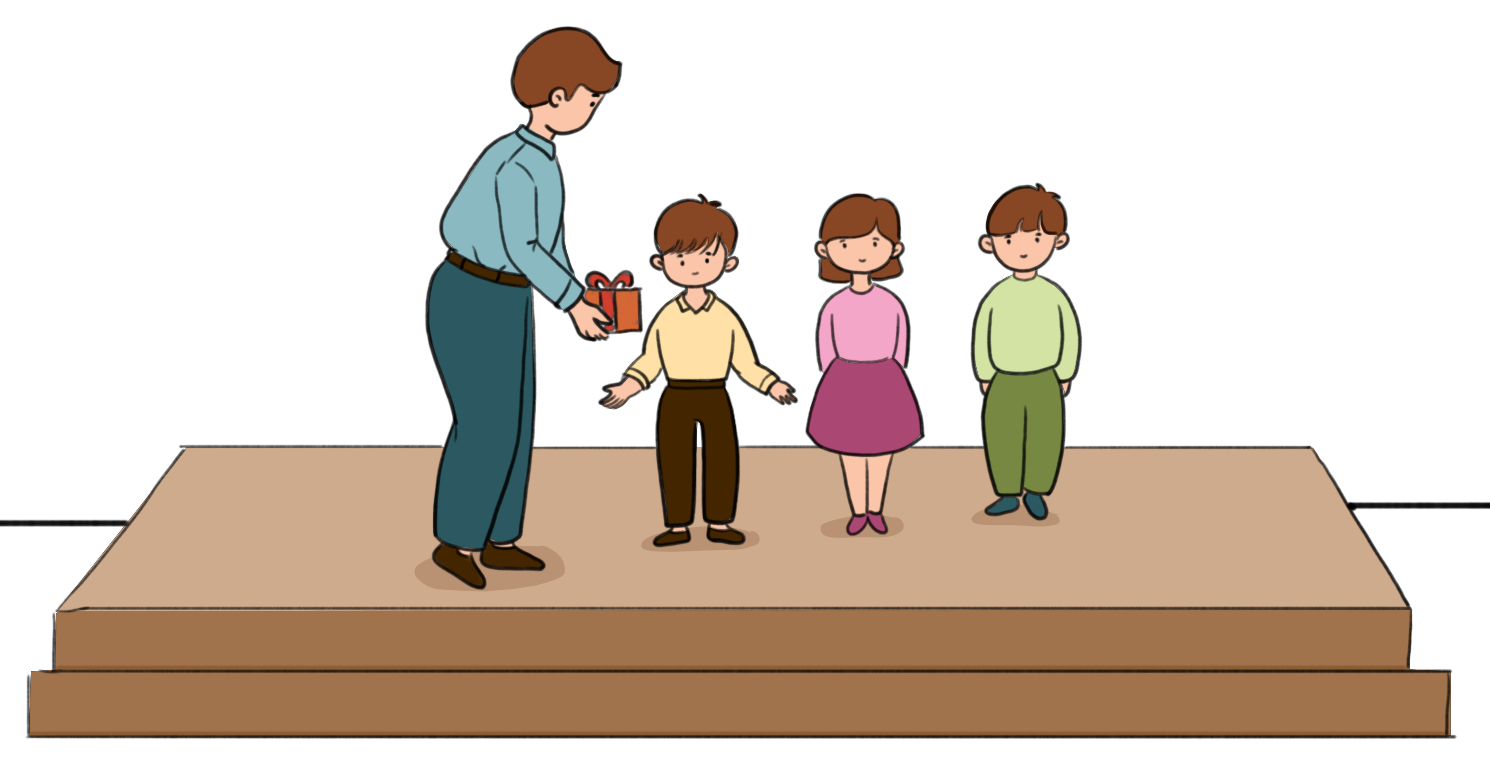
\includegraphics[width=1\linewidth]{Hinh3}
%		\vspace*{-15pt}
%	\end{figure}
%	\textit{Lời giải.} 	Số $252$ được phân tích ra các thừa số như sau: $252=4\cdot 63=7\cdot 36=11\cdot 22+10$.
%	\vskip 0.1cm
%	Vậy có $63$ em  đứng ở vị trí $4,8,12,\ldots$; có $36$ em đứng ở vị trí $7, 14, 21,\ldots$; có $22$ em đứng ở vị trí $11, 22, 33,\ldots$
%	\vskip 0.1cm
%	Do $252=28\cdot 9=44\cdot 5+32= 77\cdot 3+21$ nên có $9$ em học sinh đã được nhận quà từ nhà tài trợ thứ nhất và thứ hai, có $5$ em nhận quà từ nhà tài trợ thứ hai và ba, và $3$ em nhận quà từ nhà tài trợ thứ ba và thứ nhất. Ngoài ra không có em nào nhận quà từ cả ba nhà tài trợ này.
%	\vskip 0.1cm
%	Suy ra số học sinh đã nhận quà từ ba nhà tài trợ thứ nhất, thứ hai, thứ ba là 
%	\begin{align*}
%		63+36+22-(9+5+3)=104 \text{ (em)}.
%	\end{align*}
%	Vậy số em nhận quà từ nhà tài trợ thứ tư là $252-104=148$ (em).
%	\vskip 0.1cm
%	Tóm tại số học sinh được nhận quà từ các nhà tài trợ thứ nhất, hai, ba, tư lần lượt là $63$, $36$, $22$ và $148$.
%	\vskip 0.1cm
%	$\pmb{4.}$ 	Có ba nhà tài trợ quyết định giúp đỡ một tạp chí khoa học thường thức với tên gọi là Phi. Nhà tài trợ Quốc trao tặng một khoản tiền tính bằng dollar gồm có $4$ chữ số: $2$ chữ số đứng trước dấu phẩy, và hai chữ số sau dấu phẩy, trong đó số cent lẻ (tức là hai chữ số đứng sau dấu phẩy) bằng với đúng số dollar chẵn (tức là hai chữ số đứng trước dấu phẩy; ta nhớ lại $100$ cent $= 1$ dollar). Nhà tài trợ Minh tặng số tiền với số dollar chẵn lớn hơn $3$ dollar so với số dollar chẵn mà nhà tài trợ Quốc đã tặng nhưng số cent lẻ lại ít hơn $8$ lần số cent lẻ của nhà tài trợ Quốc. Nhà tài trợ Vũ hào phóng đem tặng số tiền bằng $1/7$ tổng số tiền của hai nhà tài trợ Quốc và Minh đã trao cộng lại. Hỏi số tiền ủng hộ của ba nhà tài trợ cho tạp chí Phi là bao nhiêu?
%	\begin{figure}[H]
%		\centering
%		\vspace*{-5pt}
%		\captionsetup{labelformat= empty, justification=centering}
%		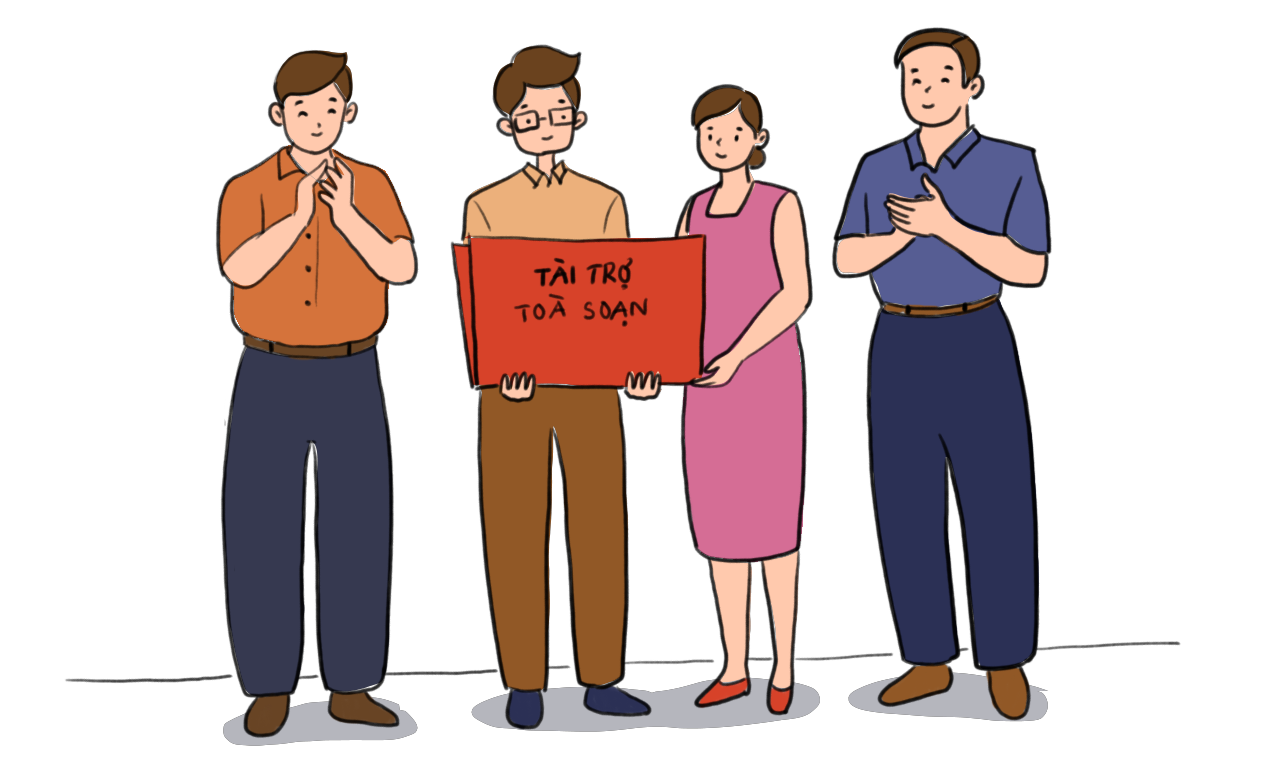
\includegraphics[width=0.85\linewidth]{Hinh4}
%		\vspace*{-10pt}
%	\end{figure}
%	\textit{Lời giải.} 	Giả sử nhà tài trợ Quốc đã tặng $x$ dollar chẵn và $x$ cent. Ta thấy $x$ không thể lớn hơn $99$. Khi đó nhà tài trợ Minh đã tặng $x+3$ dollar và $x/8$ cent. Từ đây suy ra $x$ chia hết cho $8$. Có nghĩa là $x=8y$, với $y$ không vượt quá $12$.
%	\vskip 0.1cm
%	Tổng số tiền hai nhà tài trợ Quốc và Minh tặng tạp chí Phi là $16y+3$ dollar và $9y$ cent, đổi ra cent là $1609y+300$ (cent).
%	\vskip 0.1cm
%	Số này viết được ở dạng $7(230y+43)-(y+1)$, suy ra $y+1$ chia hết cho $7$ để tổng số tiền của hai nhà tài trợ Quốc và Minh đã tặng chia hết cho $7$ (ta nhớ lại rằng nhà tài trợ Vũ đã tặng số tiền bằng $\dfrac{1}{7}$ tổng số tiền của ông Quốc và ông Minh). Trong số các số từ $1$ tới $12$, chỉ có duy nhất $y=6$ là thoả mãn điều kiện này.
%	\vskip 0.1cm
%	Vậy $x= 48$.
%	\vskip 0.1cm
%	Cuối cùng, ta thấy nhà tài trợ Quốc đã tặng tạp chí $48.48$ dollar, nhà tài trợ Minh đã tặng $51.06$ dollar và nhà tài trợ Vũ đã tặng $14.22$ dollar. Tổng cộng cả ba nhà tài trợ đã tặng cho tạp chí Phi $113.76$ dollar.
%	\vskip 0.1cm
%	$\pmb{5.}$ 	Trên hòn đảo Ngọc ở giữa một đại dương xanh ngắt có $100$ thổ dân sinh sống, một số người trong họ luôn nói dối, còn những người còn lại luôn nói thật. Mỗi một thổ dân thờ phụng đúng một trong ba vị thần: thần Mặt trời, thần Mặt trăng hoặc thần Đất. Người ta hỏi mỗi thổ dân ba câu hỏi sau đây:
%	\begin{figure}[H]
%		\centering
%		\vspace*{-5pt}
%		\captionsetup{labelformat= empty, justification=centering}
%		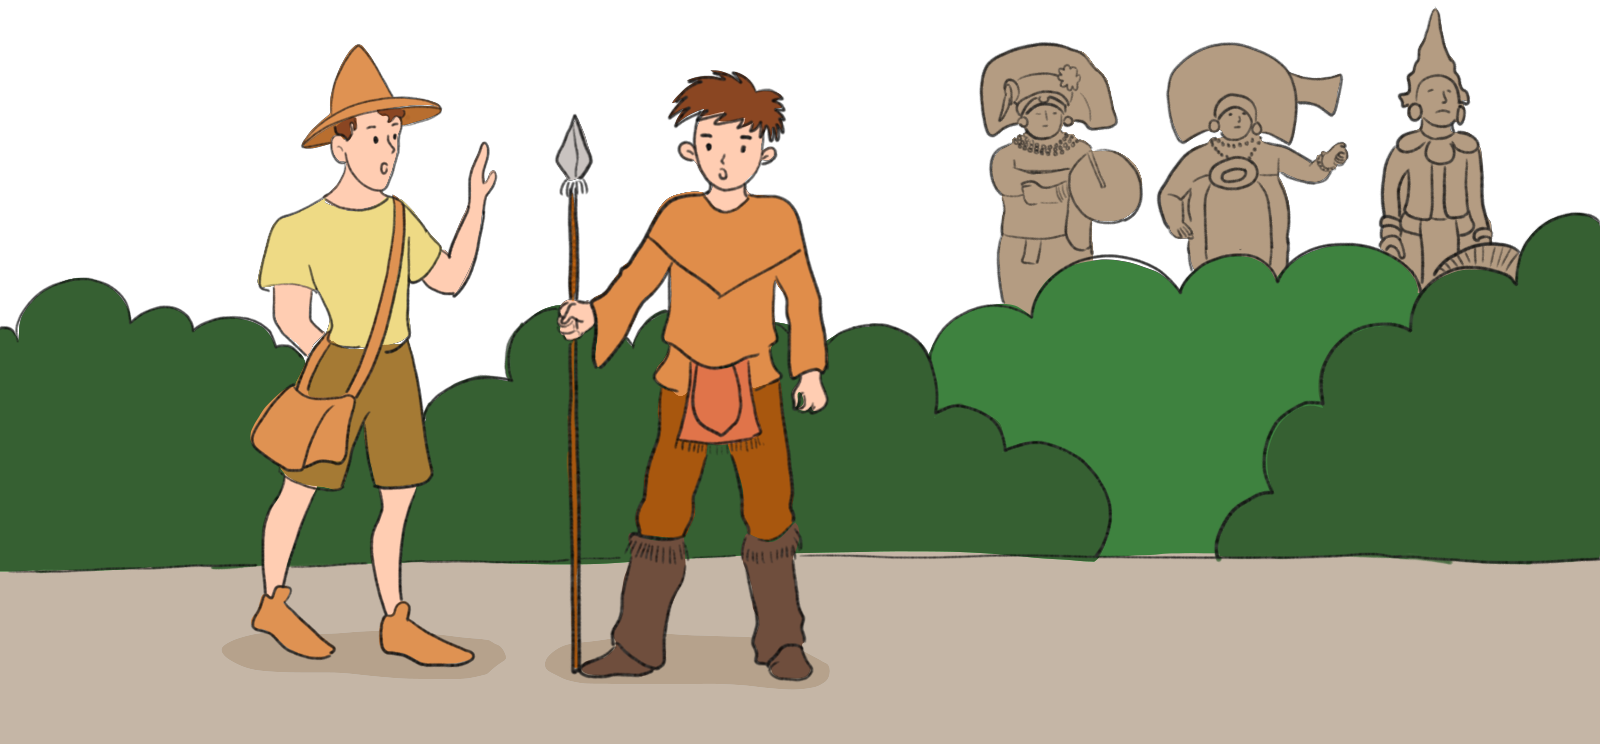
\includegraphics[width=1\linewidth]{Hinh5}
%		\vspace*{-20pt}
%	\end{figure}
%	$1.$ Ông (bà) có thờ phụng thần Mặt trời hay không?
%	\vskip 0.1cm
%	$2.$ Ông (bà) có thờ phụng thần Mặt trăng hay không?
%	\vskip 0.1cm
%	$3.$ Ông (bà) có thờ phụng thần Đất hay không?
%	\vskip 0.1cm
%	Có $60$ người trả lời khẳng định ``có" với câu hỏi thứ nhất, $40$ người trả lời khẳng định ``có" với câu hỏi thứ hai và $30$ người trả lời khẳng định ``có" với câu hỏi thứ ba. Hỏi trên đảo Ngọc có bao nhiêu thổ dân nói dối?
%	\vskip 0.1cm
%	\textit{Lời giải.} 	Mỗi người nói dối sẽ đưa ra câu trả lời ``có" tận hai lần cho ba câu hỏi, còn những người nói thật sẽ chỉ trả lời ``có" đúng một lần. Tổng cộng có $130$ lần nhận được câu trả lời là ``có", mà số thổ dân là $100$, nên số người trả lời ``có" hai lần sẽ là $130-100= 30$ (người). 
%	\vskip 0.1cm
%	Đáp số: $30$ người nói dối.
%	\vskip 0.1cm
%	$\pmb{6.}$ 	Có $100$ em học sinh được mời tới buổi tổng kết cuối năm học của nhà trường. Các ghế trong phòng họp được xếp ngay ngắn thẳng hàng theo dạng một hình vuông với $10$ dãy ghế, mỗi dãy có đúng $10$ chiếc ghế. Buổi họp phải diễn ra muộn hơn do bị cắt điện, vì thế các em học sinh bắt đầu bàn luận trao đổi với các bạn bên cạnh về kết quả điểm trung bình của mình. Em học sinh nào thấy trong tất cả những bạn ngồi kề sát mình: bên trái, bên phải, đằng sau, đằng trước và theo các đường chéo, chỉ có tối đa một bạn có điểm trung bình cao hơn hoặc bằng điểm trung bình của  mình, sẽ tự coi mình là ``có thành tích".
%	\begin{figure}[H]
%		\centering
%		\vspace*{-10pt}
%		\captionsetup{labelformat= empty, justification=centering}
%		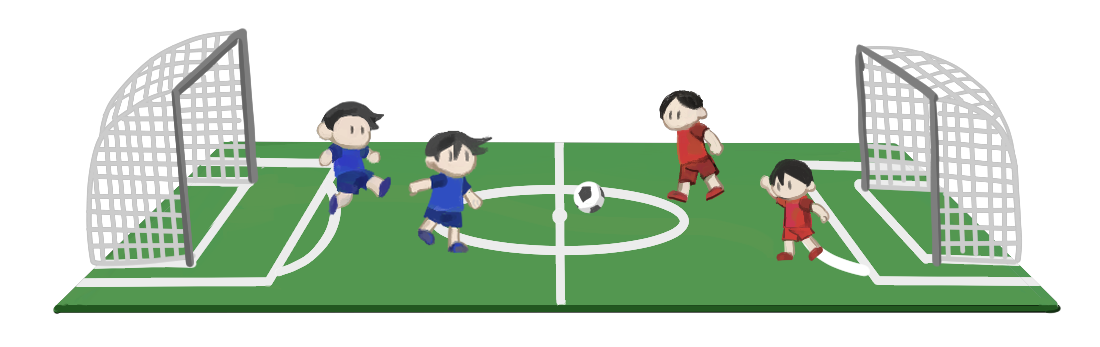
\includegraphics[width=0.85\linewidth]{Hinh6}
%		\vspace*{-10pt}
%	\end{figure}
%	Hỏi trong buổi họp đó có thể có tối đa bao nhiêu em học sinh đã tự coi mình là ``có thành tích" trong học tập?
%	\vskip 0.1cm
%	\textit{Lời giải.} Ta chia hình vuông $10\times10$ thành $25$ hình vuông nhỏ $2\times2$. Rõ ràng, trong mỗi hình vuông nhỏ như vậy chỉ có tối đa $2$ em học sinh tự coi mình ``có thành tích" trong học tập, do đó số các em học sinh như vậy không quá $50$ em. 
%	\vskip 0.1cm
%	Ta chỉ ra ví dụ về điểm trung bình của các em học sinh và cách sắp xếp các em ngồi tại các ghế trong phòng họp, hơn nữa có đúng $50$ em tự coi mình ``có thành tích" trong học tập (đó là các em có điểm trung bình khác $0$).
%	\vskip 0.2cm
%	\resizebox{\columnwidth}{!}{\begin{tabular}{|c|c|c|c|c|c|c|c|c|c|}
%		\hline
%		$1$&$0$&$1$&$0$&$1$&$0$&$1$&$0$&$1$&$0$\\
%		\hline
%		$2$&$0$&$2$&$0$&$2$&$0$&$2$&$0$&$2$&$0$\\
%		\hline
%		$3$&$0$&$3$&$0$&$3$&$0$&$3$&$0$&$3$&$0$\\
%		\hline
%		$4$&$0$&$4$&$0$&$4$&$0$&$4$&$0$&$4$&$0$\\
%		\hline
%		$5$&$0$&$5$&$0$&$5$&$0$&$5$&$0$&$5$&$0$\\
%		\hline
%		$6$&$0$&$6$&$0$&$6$&$0$&$6$&$0$&$6$&$0$\\
%		\hline
%		$7$&$0$&$7$&$0$&$7$&$0$&$7$&$0$&$7$&$0$\\
%		\hline
%		$8$&$0$&$8$&$0$&$8$&$0$&$8$&$0$&$8$&$0$\\
%		\hline
%		$9$&$0$&$9$&$0$&$9$&$0$&$9$&$0$&$9$&$0$\\
%		\hline
%		$10$&$0$&$10$&$0$&$10$&$0$&$10$&$10$&$10$&$0$\\
%		\hline
%	\end{tabular}}
%	\vspace*{1pt}
%\end{multicols}
%%
%%\newpage
%%\thispagestyle{empty}
%%\begingroup
%%\blfootnote{$^1$\color{toancuabi}Theo https://www.idm314.org/2023-comic-challenge}
%%\blfootnote{$^2$\color{toancuabi}Trường Đại Học Texas, Austin (TX), Hoa Kỳ}
%%\AddToShipoutPicture*{\put(170,680){
\includegraphics[scale=1]{../tieudehihi.pdf}}} 
%%\centering
%%\endgroup
%%\vspace*{15pt}
%%
%%\begin{figure}[H]
%%	\vspace*{5pt}
%%	\centering
%%	\captionsetup{labelformat= empty, justification=centering}
%%	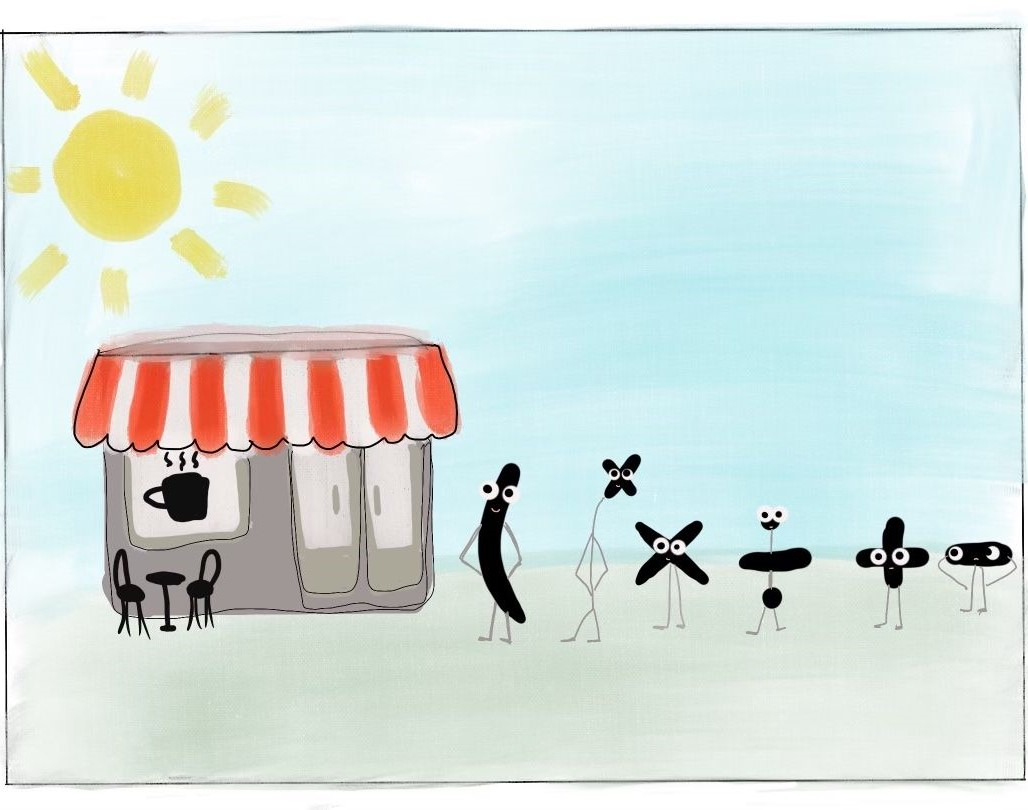
\includegraphics[width= 1\linewidth]{caphe}
%%%	\caption{\small\textit{\color{}}}
%%	\vspace*{-10pt}
%%\end{figure}
%%Các con dấu xếp hàng chờ cà phê để bắt đầu công việc của mình. Luôn phải chờ đợi theo thứ tự này. 
%%
%%\newpage
%%\thispagestyle{empty}
%%\begingroup
%%\blfootnote{$^1$\color{toancuabi}Istituto comprensivo Silvio D'arzo settore tecnico grafico Reggio Emilia (Emilia Romagna, Italia Reggio, Emilia ), Italy.}
%%\blfootnote{$^2$\color{toancuabi}Stadium là đơn vị độ dài, bằng độ dài một sân vận động thời Hy Lạp--La Mã, vào khoảng $156$ mét.}
%%\AddToShipoutPicture*{\put(126,650){
\includegraphics[scale=1]{../tieudehihi2.pdf}}} 
%%\centering
%%\endgroup
%%\vspace*{50pt}
%%
%%\begin{figure}[H]
%%	\vspace*{5pt}
%%	\centering
%%	\captionsetup{labelformat= empty, justification=centering}
%%	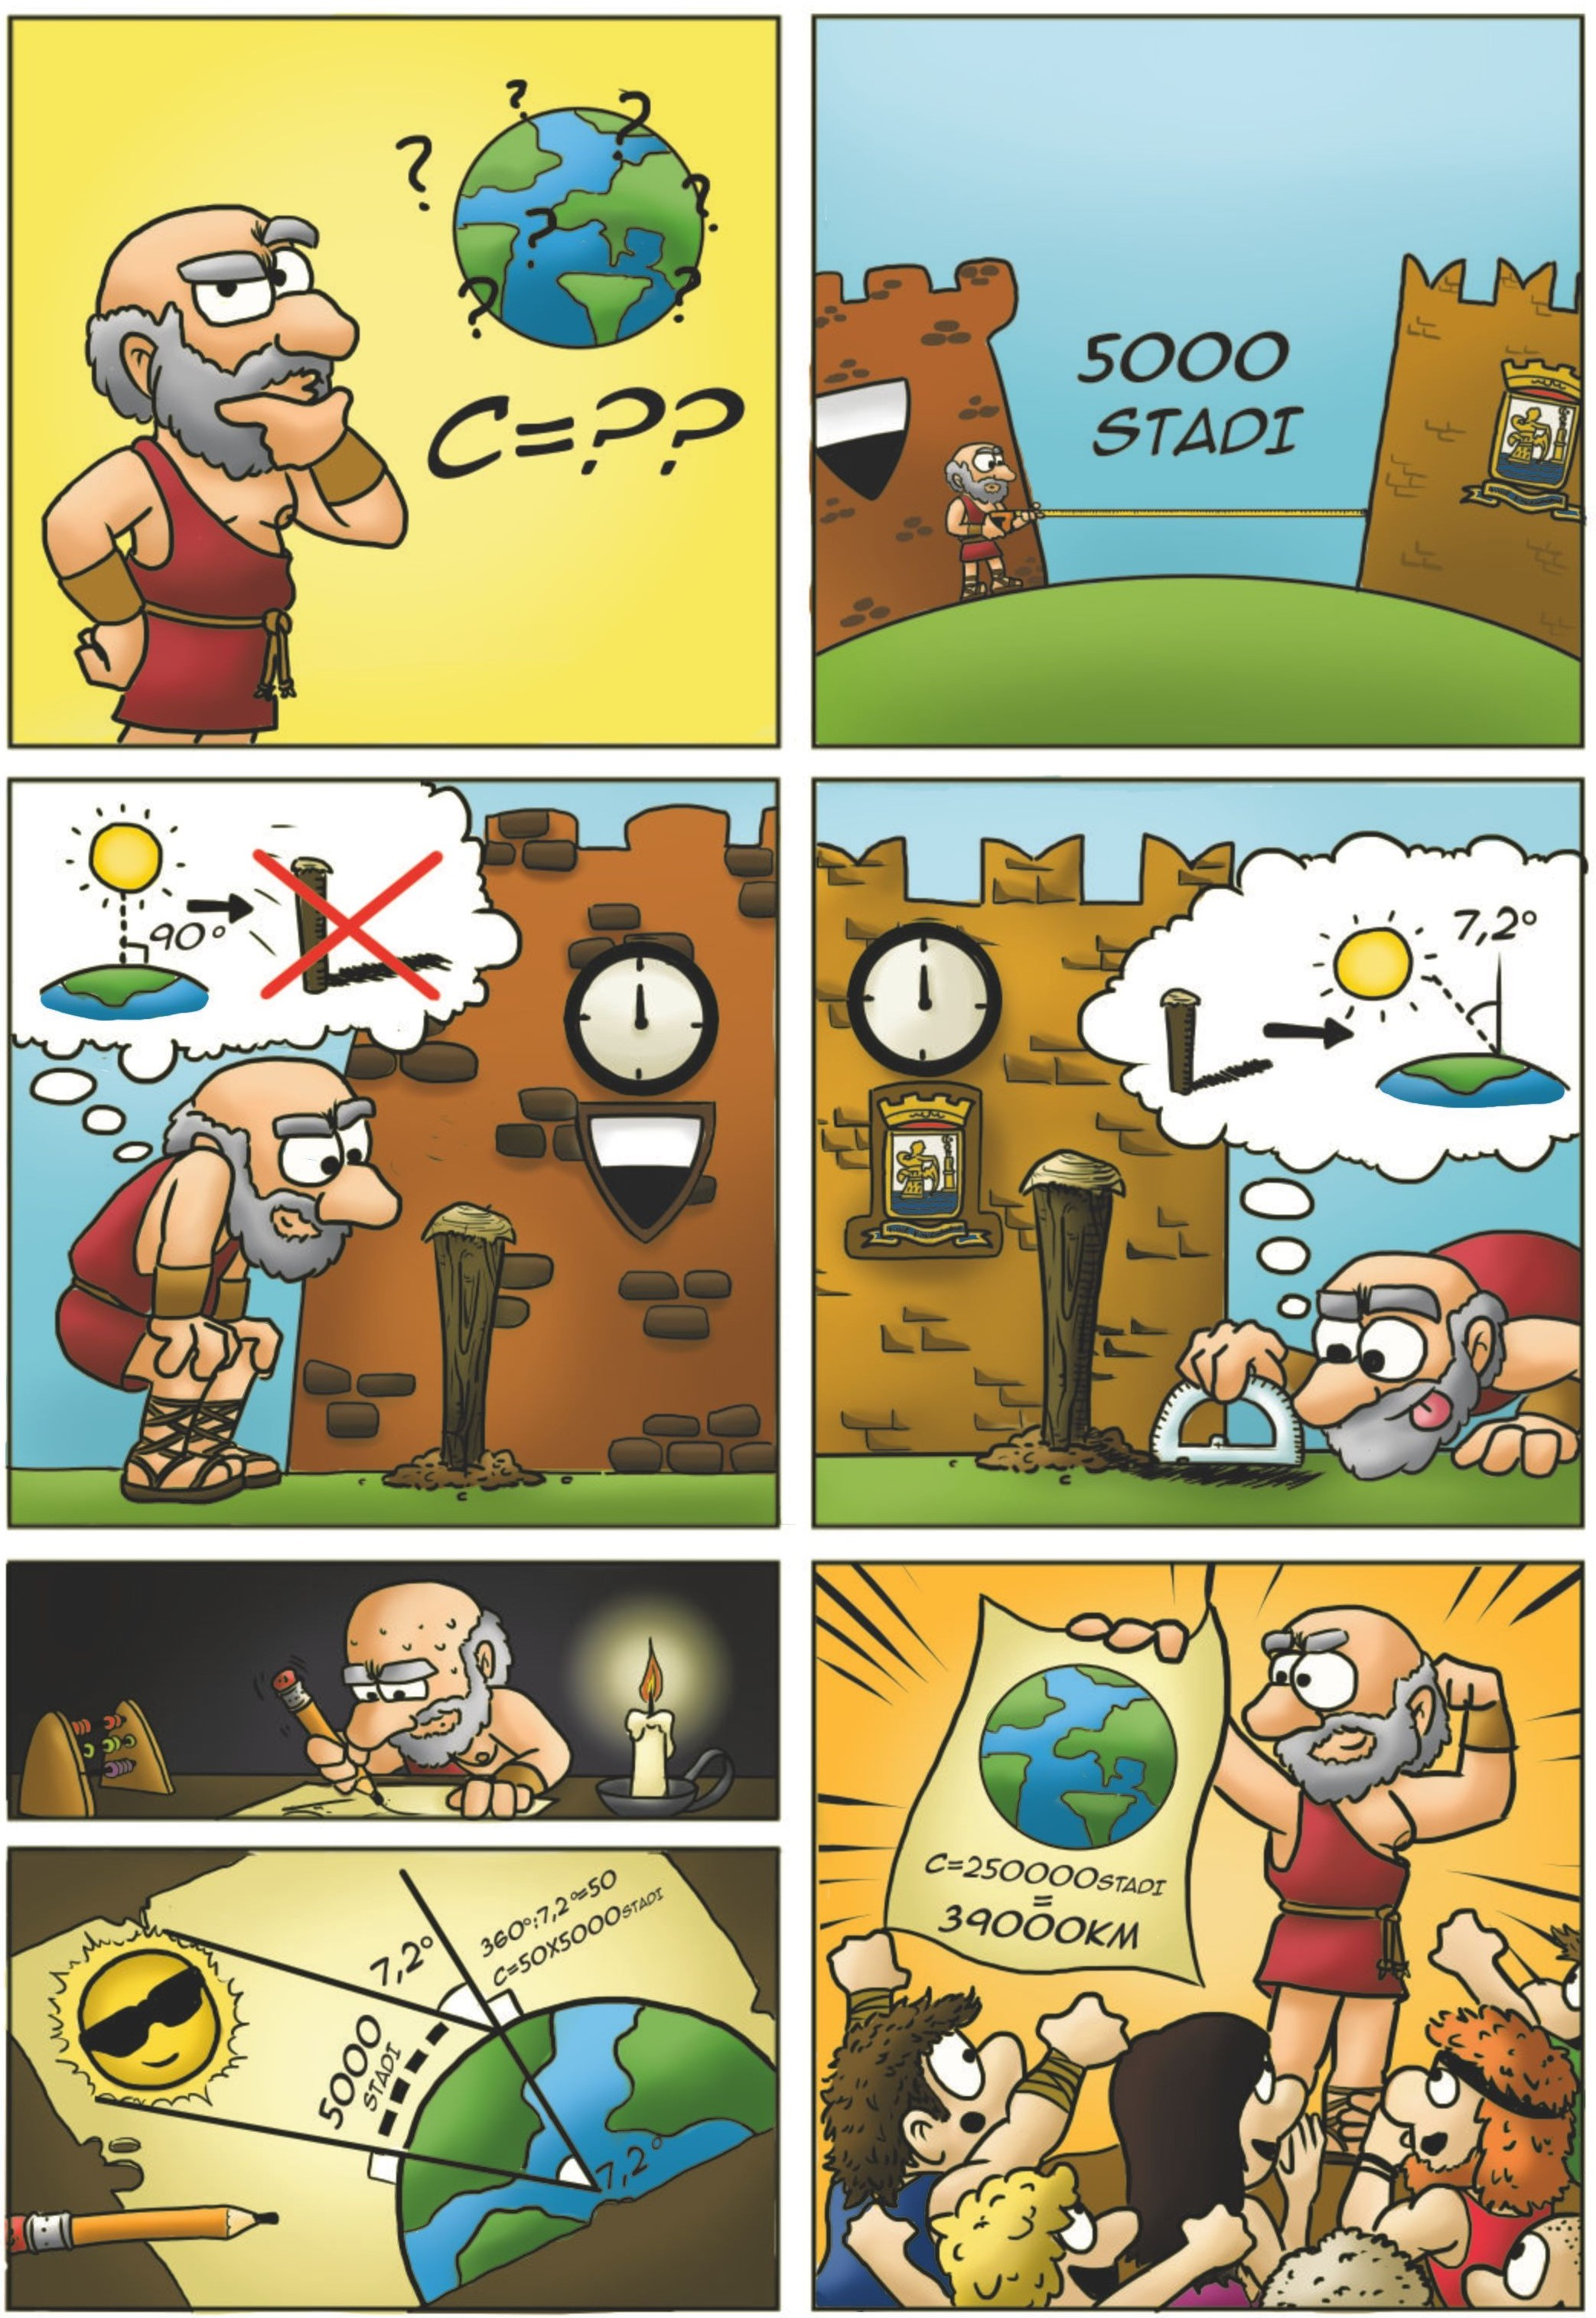
\includegraphics[width= 0.75\linewidth]{320}
%%	%	\caption{\small\textit{\color{}}}
%%	\vspace*{-10pt}
%%\end{figure}
%%Khoảng cách giữa Siena và Alexandria là $5000$ stadium$^2$  và vào giữa ngày hạ chí ở Siena, mặt trời chiếu vuông góc với trái đất trong khi ở Alexandria nó nghiêng $7{,}2^\circ$. Do đó ông đã tính chu vi Trái Đất xuống tương đương $7{,}2:360=5000:x$.
%
%
%
%\newpage
%\graphicspath{{../toancuabi/toantienganh/}}
%\begingroup
%\thispagestyle{toancuabinone}
%\blfootnote{$^1$\color{toancuabi}Ottawa, Canada.}
%\AddToShipoutPicture*{\put(60,733){
\includegraphics[width=17.2cm]{../mathc.pdf}}}
%%\AddToShipoutPicture*{\put(-2,733){
\includegraphics[width=17.2cm]{../mathl.pdf}}} 
%\AddToShipoutPicture*{\put(66,670){
\includegraphics[scale=1]{../tieudeb.pdf}}} 
%\centering
%\endgroup
%\vspace*{40pt}
%
%\begin{multicols}{2}
%	This article is the second part of the series on demonstration \textit{Proof by Contradiction}.
%	\vskip 0.2cm
%	\PIbox{
%	\textbf{\color{toancuabi}\color{toancuabi}\color{toancuabi}\color{toancuabi}Example $\pmb6$.}
%	Twenty--five persons from $8$ different provinces elected to the National Congress.
%	Prove that at least $4$ of them are from the same province.}
%	\vskip 0.2cm
%	\textit{Solution.}
%	Assume that this is not true. Then no $4$ of them are from the same province.
%	In this case, not more than $3$ persons are from the $1^{\text{st}}$ province, not more than $3$ from the $2^{\text{nd}}$, and so on.
%	Altogether, there are not more than $3 \times 8 = 24$ persons. This contradicts the fact that there are $25$ persons.
%	\vskip 0.2cm
%	\PIbox{\textbf{\color{toancuabi}\color{toancuabi}\color{toancuabi}\color{toancuabi}Example $\pmb7$.}
%	At the graduation event of the School of Wizardry, $5$ outstanding students called to the podium.
%	They standing in a row. Altogether, these $5$ students know $300$ different spells.
%	Prove that there are $2$ students standing next to each other who, if combined, know at least $100$ spells.}
%	\vskip 0.1cm
%	\textit{Solution.}
%	Suppose that this is not true. Then the $1^{\text{st}}$ and $2^{\text{nd}}$ students together know less than $100$ spells,
%	and the $4^{\text{th}}$ and $5^{\text{th}}$ students together know less than $100$ spells.
%	Then these four know less than $200$ spells together. In this case, the $3^{\text{rd}}$ student knows more than $100$ spells.
%	\vskip 0.2cm
%	\PIbox{\textbf{\color{toancuabi}\color{toancuabi}\color{toancuabi}\color{toancuabi}Example $\pmb8$.}
%	The only way to travel in the Kingdom of so many swamps is to use magic carpets.
%		Twenty--one carpet--transportation \,lines \,\,serve \,\,the \,\,capital. \,A 
%	}
%	
%	\PIbox{single carpet--transportation line goes to Tinyville, and every other city is served by exactly $20$ carpet--transportation lines.
%		Show that it is possible to travel by magic carpet from the capital to Tinyville (perhaps by transferring from one carpet line to another).}
%	\vskip 0.2cm
%	\textit{Solution.} Let's take a look at all the cities that are accessible by magic carpet from Tinyville. The capital does not belong to this group. In this group there is a number of cities, each has $20$ lines leading to it,
%		and one city (Tinyville) with only one line leading to it. Thus the sum of all lines leading to the cities is an odd number.
%		But this is not true. If we count the lines among these cities, then they have to be counted twice, thus it is an even number.
%		This contradiction means Tinyville is connected to the capital.
%	\vskip 0.2cm
%	\PIbox{\textbf{\color{toancuabi}\color{toancuabi}\color{toancuabi}\color{toancuabi}Example $\pmb9$.}
%		The game of Trick--a--Troll is played with $10$ players and a deck of $20$ cards:
%		$2$ through $10$ and an ace of spades, and $2$ through $10$ and an ace of clubs.
%		Each player gets $1$ club and $1$ spade and adds his cards (aces count as $1$).
%		Prove that there will be at least $2$ players with sums that end in the same digit.}
%	\vskip 0.2cm
%	\textit{Solution.}
%	Let's consider the sum of the values of all the cards.
%	If we assume that all players had different last digits for their sums, then all $10$ digits would be present, and the sum of them all would end with a $5$.
%	On the other hand, the sum of the values of all cards in play ends with a $0$, a contradiction.
%	\vskip 0.2cm
%	\PIbox{\textbf{\color{toancuabi}\color{toancuabi}\color{toancuabi}\color{toancuabi}Example $\pmb10$.}
%	At each of the vertices of a regular hexagon there stands a grasshopper.
%		At the same time, all six grasshoppers jump off the ground. They land at the same time,
%		each at one of the vertices. No two grasshoppers land at the same vertex.
%		Each of the grasshoppers does not necessarily land at a vertex different from the one it jumps off.
%		Prove that there exist three grasshoppers jump off vertices $A, B,$ and $C,$
%		and land at $A', B'$ and $C',$ such that $\triangle ABC$ and $\triangle A'B'C'$ are congruent.}
%	\vskip 0.2cm
%	\textit{Solution.}
%		Let assume that it is not possible for such scenario. In other words, if any three grasshoppers jump off vertices $A, B,$ and $C,$
%		and land at $A', B'$ and $C',$ then $\triangle ABC$ and $\triangle A'B'C'$ \textit{are not congruent.}
%		\vskip 0.1cm
%		First, we find out how many types of triangles can be constructed with three vertices of the hexagon.
%		There are three types of triangles, such that \textit{they are pair--wise not congruent}, see the diagram below.
%	\begin{figure}[H]
%		\vspace*{-5pt}
%		\centering
%		\captionsetup{labelformat= empty, justification=centering}
%		\begin{tikzpicture}[toancuabi, scale = 0.4 scale=0.4, node font=\scriptsize]
%			\fill[fill=cackithi!40] (3.8660254037844397,2.767949192431121) -- (2.,4.) -- (0.,3.) -- cycle;
%			\fill[fill=cackithi!40] (9.732050807568879,0.5358983848622445) -- (9.866025403784441,2.7679491924311215) -- (6.,3.) -- cycle;
%			\fill[fill=cackithi!40] (15.866025403784441,2.7679491924311215) -- (13.732050807568879,-0.4641016151377553) -- (12.,3.) -- cycle;
%			\draw  (2.,4.)-- (0.,3.);
%			\draw  (0.,3.)-- (-0.13397459621556163,0.7679491924311225);
%			\draw  (-0.13397459621556163,0.7679491924311225)-- (1.7320508075688774,-0.4641016151377553);
%			\draw  (1.7320508075688774,-0.4641016151377553)-- (3.7320508075688776,0.5358983848622443);
%			\draw  (3.7320508075688776,0.5358983848622443)-- (3.8660254037844397,2.767949192431121);
%			\draw  (3.8660254037844397,2.767949192431121)-- (2.,4.);
%			\draw  (8.,4.)-- (6.,3.);
%			\draw  (6.,3.)-- (5.866025403784439,0.7679491924311221);
%			\draw  (5.866025403784439,0.7679491924311221)-- (7.7320508075688785,-0.4641016151377553);
%			\draw  (7.7320508075688785,-0.4641016151377553)-- (9.732050807568879,0.5358983848622445);
%			\draw  (9.732050807568879,0.5358983848622445)-- (9.866025403784441,2.7679491924311215);
%			\draw  (9.866025403784441,2.7679491924311215)-- (8.,4.);
%			\draw  (14.,4.)-- (12.,3.);
%			\draw  (12.,3.)-- (11.86602540378444,0.7679491924311221);
%			\draw  (11.86602540378444,0.7679491924311221)-- (13.732050807568879,-0.4641016151377553);
%			\draw  (13.732050807568879,-0.4641016151377553)-- (15.732050807568879,0.5358983848622445);
%			\draw  (15.732050807568879,0.5358983848622445)-- (15.866025403784441,2.7679491924311215);
%			\draw  (15.866025403784441,2.7679491924311215)-- (14.,4.);
%			\draw  (3.8660254037844397,2.767949192431121)-- (2.,4.);
%			\draw  (2.,4.)-- (0.,3.);
%			\draw  (0.,3.)-- (3.8660254037844397,2.767949192431121);
%			\draw  (9.732050807568879,0.5358983848622445)-- (9.866025403784441,2.7679491924311215);
%			\draw  (9.866025403784441,2.7679491924311215)-- (6.,3.);
%			\draw  (6.,3.)-- (9.732050807568879,0.5358983848622445);
%			\draw  (15.866025403784441,2.7679491924311215)-- (13.732050807568879,-0.4641016151377553);
%			\draw  (13.732050807568879,-0.4641016151377553)-- (12.,3.);
%			\draw  (12.,3.)-- (15.866025403784441,2.7679491924311215);
%			\draw  (-1.,5.)-- (17.,5.);
%			\draw  (17.,5.)-- (17.,-2.);
%			\draw  (17.,-2.)-- (-1.,-2.);
%			\draw  (-1.,-2.)-- (-1.,5.);
%			\draw  (5.,5.)-- (5.,-2.);
%			\draw  (11.,5.)-- (11.,-2.);
%			\draw  (-1.,-1.)-- (17.,-1.);
%			\draw [fill=white] (2.,4.) circle (2.0pt);
%			\draw (2.14,4.37) node {$A$};
%			\draw [fill=white] (0.,3.) circle (2.0pt);
%			\draw (-0.16,3.33) node {$B$};
%			\draw [fill=white] (-0.13397459621556163,0.7679491924311225) circle (2.0pt);
%			\draw (-0.4,0.61) node {$C$};
%			\draw [fill=white] (1.7320508075688774,-0.4641016151377553) circle (2.0pt);
%			\draw (2.02,-0.63) node {$D$};
%			\draw [fill=white] (3.7320508075688776,0.5358983848622443) circle (2.0pt);
%			\draw (4.04,0.41) node {$E$};
%			\draw [fill=white] (3.8660254037844397,2.767949192431121) circle (2.0pt);
%			\draw (4.08,3.15) node {$F$};
%			\draw [fill=white] (8.,4.) circle (2.0pt);
%			\draw (8.14,4.37) node {$G$};
%			\draw [fill=white] (6.,3.) circle (2.0pt);
%			\draw (5.78,3.41) node {$H$};
%			\draw [fill=white] (5.866025403784439,0.7679491924311221) circle (2.0pt);
%			\draw (5.6,0.65) node {$I$};
%			\draw [fill=white] (7.7320508075688785,-0.4641016151377553) circle (2.0pt);
%			\draw (8.04,-0.59) node {$J$};
%			\draw [fill=white] (9.732050807568879,0.5358983848622445) circle (2.0pt);
%			\draw (9.94,0.29) node {$K$};
%			\draw [fill=white] (9.866025403784441,2.7679491924311215) circle (2.0pt);
%			\draw (10.06,3.13) node {$L$};
%			\draw [fill=white] (14.,4.) circle (2.0pt);
%			\draw (14.,4.43) node {$M$};
%			\draw [fill=white] (12.,3.) circle (2.0pt);
%			\draw (11.74,3.31) node {$N$};
%			\draw [fill=white] (11.86602540378444,0.7679491924311221) circle (2.0pt);
%			\draw (11.62,0.49) node {$O$};
%			\draw [fill=white] (13.732050807568879,-0.4641016151377553) circle (2.0pt);
%			\draw (14.14,-0.65) node {$P$};
%			\draw [fill=white] (15.732050807568879,0.5358983848622445) circle (2.0pt);
%			\draw (15.94,0.31) node {$Q$};
%			\draw [fill=white] (15.866025403784441,2.7679491924311215) circle (2.0pt);
%			\draw (16.1,3.05) node {$R$};
%			\draw[color=black] (2,-1.6) node {$\text{Type } 1$};
%			\draw[color=black] (8,-1.6) node {$\text{Type } 2$};
%			\draw[color=black] (14,-1.6) node {$\text{Type }3$};
%		\end{tikzpicture}
%		\vspace*{-10pt}
%	\end{figure}
%		For \textit{Type $1$}, there are $6$ such triangles; for \textit{Type $2$}, $12$ triangles,; and for \textit{Type $3$}, $2$ triangles.
%		(there are $20$ such triangles in total.) 
%		\vskip 0.1cm
%		Now, our assumption means that $12$ triangles of Type $2$ should be change to the same number of distinct triangles of Type $1$ or Type $2$,
%		which is impossible since there are only $6+2=8$ of them. This is a contradiction.
%\end{multicols}
